\documentclass[a4paper]{book}
\usepackage{a4wide}
\usepackage{makeidx}
\usepackage{graphicx}
\usepackage{multicol}
\usepackage{float}
\usepackage{listings}
\usepackage{color}
\usepackage{textcomp}
\usepackage{alltt}
\usepackage{times}
\usepackage{ifpdf}
\ifpdf
\usepackage[pdftex,
            pagebackref=true,
            colorlinks=true,
            linkcolor=blue,
            unicode
           ]{hyperref}
\else
\usepackage[ps2pdf,
            pagebackref=true,
            colorlinks=true,
            linkcolor=blue,
            unicode
           ]{hyperref}
\usepackage{pspicture}
\fi
\usepackage[utf8]{inputenc}
\usepackage{doxygen}
\lstset{language=C++,inputencoding=utf8,basicstyle=\footnotesize,breaklines=true,breakatwhitespace=true,tabsize=8,numbers=left }
\makeindex
\setcounter{tocdepth}{3}
\renewcommand{\footrulewidth}{0.4pt}
\begin{document}
\hypersetup{pageanchor=false}
\begin{titlepage}
\vspace*{7cm}
\begin{center}
{\Large celib \\[1ex]\large Version 0.0.1 }\\
\vspace*{1cm}
{\large Generated by Doxygen 1.6.1}\\
\vspace*{0.5cm}
{\small Thu Dec 31 18:44:34 2009}\\
\end{center}
\end{titlepage}
\clearemptydoublepage
\pagenumbering{roman}
\tableofcontents
\clearemptydoublepage
\pagenumbering{arabic}
\hypersetup{pageanchor=true}
\chapter{Data Structure Index}
\section{Data Structures}
Here are the data structures with brief descriptions:\begin{DoxyCompactList}
\item\contentsline{section}{\hyperlink{struct___ce_string}{CeString} }{\pageref{struct___ce_string}}{}
\item\contentsline{section}{\hyperlink{struct___ce_string_p}{CeStringP} }{\pageref{struct___ce_string_p}}{}
\end{DoxyCompactList}

\chapter{File Index}
\section{File List}
Here is a list of all files with brief descriptions:\begin{DoxyCompactList}
\item\contentsline{section}{src/\hyperlink{celib_8h}{celib.h} }{\pageref{celib_8h}}{}
\item\contentsline{section}{src/\hyperlink{cemacros_8h}{cemacros.h} }{\pageref{cemacros_8h}}{}
\item\contentsline{section}{src/\hyperlink{cestring_8c}{cestring.c} }{\pageref{cestring_8c}}{}
\item\contentsline{section}{src/\hyperlink{cestring_8h}{cestring.h} }{\pageref{cestring_8h}}{}
\item\contentsline{section}{src/\hyperlink{ceswap_8c}{ceswap.c} }{\pageref{ceswap_8c}}{}
\item\contentsline{section}{src/\hyperlink{ceswap_8h}{ceswap.h} }{\pageref{ceswap_8h}}{}
\item\contentsline{section}{src/\hyperlink{cetypes_8h}{cetypes.h} }{\pageref{cetypes_8h}}{}
\end{DoxyCompactList}

\chapter{Data Structure Documentation}
\hypertarget{struct___ce_string}{
\section{CeString Struct Reference}
\label{struct___ce_string}\index{\_\-CeString@{\_\-CeString}}
}


{\ttfamily \#include $<$cestring.h$>$}\subsection*{Data Fields}
\begin{DoxyCompactItemize}
\item 
\hyperlink{cetypes_8h_a3a94319866313b53b54825af2ba77e8d}{CeUChar} $\ast$const \hyperlink{struct___ce_string_a5d1597aa704055227e587c70976f9edc}{data}
\item 
\hyperlink{cetypes_8h_aced3fca6c74c98a0a7c07757af07abca}{CeInt} const \hyperlink{struct___ce_string_a441d506b9271f3d6192d9973d33b97bb}{len}
\begin{DoxyCompactList}\small\item\em string length excluding trailing '' \item\end{DoxyCompactList}\end{DoxyCompactItemize}


\subsection{Detailed Description}


Definition at line 28 of file cestring.h.

\subsection{Field Documentation}
\hypertarget{struct___ce_string_a5d1597aa704055227e587c70976f9edc}{
\index{\_\-CeString@{\_\-CeString}!data@{data}}
\index{data@{data}!_CeString@{\_\-CeString}}
\subsubsection[{data}]{\setlength{\rightskip}{0pt plus 5cm}{\bf CeUChar}$\ast$ const {\bf data}}}
\label{struct___ce_string_a5d1597aa704055227e587c70976f9edc}


Definition at line 29 of file cestring.h.\hypertarget{struct___ce_string_a441d506b9271f3d6192d9973d33b97bb}{
\index{\_\-CeString@{\_\-CeString}!len@{len}}
\index{len@{len}!_CeString@{\_\-CeString}}
\subsubsection[{len}]{\setlength{\rightskip}{0pt plus 5cm}{\bf CeInt} const {\bf len}}}
\label{struct___ce_string_a441d506b9271f3d6192d9973d33b97bb}


string length excluding trailing '' 

Definition at line 30 of file cestring.h.

The documentation for this struct was generated from the following file:\begin{DoxyCompactItemize}
\item 
src/\hyperlink{cestring_8h}{cestring.h}\end{DoxyCompactItemize}

\hypertarget{struct___ce_string_p}{
\section{CeStringP Struct Reference}
\label{struct___ce_string_p}\index{\_\-CeStringP@{\_\-CeStringP}}
}
\subsection*{Data Fields}
\begin{DoxyCompactItemize}
\item 
\hyperlink{cetypes_8h_a3a94319866313b53b54825af2ba77e8d}{CeUChar} $\ast$ \hyperlink{struct___ce_string_p_a712dda5f9433ebba132fec7b76e46c0b}{data}
\item 
\hyperlink{cetypes_8h_aced3fca6c74c98a0a7c07757af07abca}{CeInt} \hyperlink{struct___ce_string_p_a3b1e093b841399b8de9feb53c583451d}{len}
\begin{DoxyCompactList}\small\item\em string length excluding trailing '' \item\end{DoxyCompactList}\end{DoxyCompactItemize}


\subsection{Detailed Description}


Definition at line 35 of file cestring.c.

\subsection{Field Documentation}
\hypertarget{struct___ce_string_p_a712dda5f9433ebba132fec7b76e46c0b}{
\index{\_\-CeStringP@{\_\-CeStringP}!data@{data}}
\index{data@{data}!_CeStringP@{\_\-CeStringP}}
\subsubsection[{data}]{\setlength{\rightskip}{0pt plus 5cm}{\bf CeUChar}$\ast$ {\bf data}}}
\label{struct___ce_string_p_a712dda5f9433ebba132fec7b76e46c0b}


Definition at line 36 of file cestring.c.

Referenced by ce\_\-string\_\-get\_\-data\_\-inrange().\hypertarget{struct___ce_string_p_a3b1e093b841399b8de9feb53c583451d}{
\index{\_\-CeStringP@{\_\-CeStringP}!len@{len}}
\index{len@{len}!_CeStringP@{\_\-CeStringP}}
\subsubsection[{len}]{\setlength{\rightskip}{0pt plus 5cm}{\bf CeInt} {\bf len}}}
\label{struct___ce_string_p_a3b1e093b841399b8de9feb53c583451d}


string length excluding trailing '' 

Definition at line 37 of file cestring.c.

The documentation for this struct was generated from the following file:\begin{DoxyCompactItemize}
\item 
src/\hyperlink{cestring_8c}{cestring.c}\end{DoxyCompactItemize}

\chapter{File Documentation}
\hypertarget{celib_8h}{
\section{src/celib.h File Reference}
\label{celib_8h}\index{src/celib.h@{src/celib.h}}
}
{\ttfamily \#include $<$celib/cemacros.h$>$}\par
{\ttfamily \#include $<$celib/cetypes.h$>$}\par
{\ttfamily \#include $<$celib/cestring.h$>$}\par
Include dependency graph for celib.h:\nopagebreak
\begin{figure}[H]
\begin{center}
\leavevmode
\includegraphics[width=175pt]{celib_8h__incl}
\end{center}
\end{figure}

\hypertarget{cemacros_8h}{
\section{src/cemacros.h File Reference}
\label{cemacros_8h}\index{src/cemacros.h@{src/cemacros.h}}
}
This graph shows which files directly or indirectly include this file:\nopagebreak
\begin{figure}[H]
\begin{center}
\leavevmode
\includegraphics[width=67pt]{cemacros_8h__dep__incl}
\end{center}
\end{figure}
\subsection*{Defines}
\begin{DoxyCompactItemize}
\item 
\#define \hyperlink{cemacros_8h_ac6f2262a6c60a4cf9a53c99f4c81da41}{CE\_\-FALSE}~0
\item 
\#define \hyperlink{cemacros_8h_a5b9c3d40d570e14ba2f70b0b28a163a7}{CE\_\-TRUE}~1
\item 
\#define \hyperlink{cemacros_8h_a8e920d7c465674d8964b4195f3d32929}{\_\-CE\_\-STR}(str)~\#str
\item 
\#define \hyperlink{cemacros_8h_a701500605dee3d09e86c6eb078778b45}{CE\_\-STR}(str)~\_\-CC\_\-STR(str)
\item 
\#define \hyperlink{cemacros_8h_a38a82c277eecf6b98ddecc879f7f3ccd}{CE\_\-MAX}(x, y)~( (x) $>$ (y) ? (x) : (y) )
\item 
\#define \hyperlink{cemacros_8h_aa21be4cc4ec33d8d026045a0c02e6759}{CE\_\-MIN}(x, y)~( (x) $<$ (y) ? (x) : (y) )
\item 
\#define \hyperlink{cemacros_8h_a07134f16140b1fdd47ef0edc43efee88}{CE\_\-POWER\_\-2}(x)~( (x) $\ast$ (x) )
\item 
\#define \hyperlink{cemacros_8h_aad69937be800bbbc8d4b7f275b726a24}{CE\_\-POWER\_\-3}(x)~( (x) $\ast$ (x) $\ast$ (x) )
\item 
\#define \hyperlink{cemacros_8h_aa21f0751fd2a2d91a53b392806cda68a}{CE\_\-UPCASE}(c)~( ( (c) $>$= 'a' \&\& (c) $<$= 'z') ? ( (c) -\/ 0x20) : (c) )
\item 
\#define \hyperlink{cemacros_8h_a79b773829412d6fe9449f842dea6ee6e}{CE\_\-DOWNCASE}(c)~( ( (c) $>$= 'A' \&\& (c) $<$= 'Z') ? ( (c) + 0x20) : (c) )
\item 
\#define \hyperlink{cemacros_8h_a3f60f158ab3e6645e16e7b0021019c2b}{CE\_\-LSHIFT}(x, offset)~( (x) $<$$<$ (offset) )
\item 
\#define \hyperlink{cemacros_8h_a2e84d489a9dedce2fa1ece3657d515e1}{CE\_\-RSHIFT}(x, offset)~( (x) $>$$>$ (offset) )
\item 
\#define \hyperlink{cemacros_8h_a2b14b6a1229836b07b79b9de43f27f84}{CE\_\-NOT}(a)~( $\sim$(a) )
\item 
\#define \hyperlink{cemacros_8h_afd25210fc93077c1b93722a0d2536048}{CE\_\-OR}(a, b)~( (a) $|$ (b) )
\item 
\#define \hyperlink{cemacros_8h_a6358684cf7b38fb9f59b9fac5b2cda36}{CE\_\-AND}(a, b)~( (a) \& (b) )
\item 
\#define \hyperlink{cemacros_8h_a0c5d5771e54175e79ed993f5cceba31a}{CE\_\-XOR}(a, b)~( (a) $^\wedge$ (b) )
\item 
\#define \hyperlink{cemacros_8h_a7868dfa4a54d76195a299eb0ff5701f1}{CE\_\-NOR}(a, b)~( $\sim$( (a) $|$ (b) ) )
\item 
\#define \hyperlink{cemacros_8h_a0d4f5a97ba4162d4122cae14e0ffea2b}{CE\_\-NAND}(a, b)~( $\sim$( (a) \& (b) ) )
\item 
\#define \hyperlink{cemacros_8h_a06a5a6b41431c9af06deb287dfb76449}{CE\_\-RANGE\_\-INITIAL}(start, end, length)
\end{DoxyCompactItemize}


\subsection{Define Documentation}
\hypertarget{cemacros_8h_a8e920d7c465674d8964b4195f3d32929}{
\index{cemacros.h@{cemacros.h}!\_\-CE\_\-STR@{\_\-CE\_\-STR}}
\index{\_\-CE\_\-STR@{\_\-CE\_\-STR}!cemacros.h@{cemacros.h}}
\subsubsection[{\_\-CE\_\-STR}]{\setlength{\rightskip}{0pt plus 5cm}\#define \_\-CE\_\-STR(str)~\#str}}
\label{cemacros_8h_a8e920d7c465674d8964b4195f3d32929}


Definition at line 33 of file cemacros.h.\hypertarget{cemacros_8h_a6358684cf7b38fb9f59b9fac5b2cda36}{
\index{cemacros.h@{cemacros.h}!CE\_\-AND@{CE\_\-AND}}
\index{CE\_\-AND@{CE\_\-AND}!cemacros.h@{cemacros.h}}
\subsubsection[{CE\_\-AND}]{\setlength{\rightskip}{0pt plus 5cm}\#define CE\_\-AND(a, \/  b)~( (a) \& (b) )}}
\label{cemacros_8h_a6358684cf7b38fb9f59b9fac5b2cda36}


Definition at line 54 of file cemacros.h.\hypertarget{cemacros_8h_a79b773829412d6fe9449f842dea6ee6e}{
\index{cemacros.h@{cemacros.h}!CE\_\-DOWNCASE@{CE\_\-DOWNCASE}}
\index{CE\_\-DOWNCASE@{CE\_\-DOWNCASE}!cemacros.h@{cemacros.h}}
\subsubsection[{CE\_\-DOWNCASE}]{\setlength{\rightskip}{0pt plus 5cm}\#define CE\_\-DOWNCASE(c)~( ( (c) $>$= 'A' \&\& (c) $<$= 'Z') ? ( (c) + 0x20) : (c) )}}
\label{cemacros_8h_a79b773829412d6fe9449f842dea6ee6e}


Definition at line 45 of file cemacros.h.\hypertarget{cemacros_8h_ac6f2262a6c60a4cf9a53c99f4c81da41}{
\index{cemacros.h@{cemacros.h}!CE\_\-FALSE@{CE\_\-FALSE}}
\index{CE\_\-FALSE@{CE\_\-FALSE}!cemacros.h@{cemacros.h}}
\subsubsection[{CE\_\-FALSE}]{\setlength{\rightskip}{0pt plus 5cm}\#define CE\_\-FALSE~0}}
\label{cemacros_8h_ac6f2262a6c60a4cf9a53c99f4c81da41}


Definition at line 29 of file cemacros.h.

Referenced by ce\_\-string\_\-isequal(), and ce\_\-string\_\-isequal\_\-inrange().\hypertarget{cemacros_8h_a3f60f158ab3e6645e16e7b0021019c2b}{
\index{cemacros.h@{cemacros.h}!CE\_\-LSHIFT@{CE\_\-LSHIFT}}
\index{CE\_\-LSHIFT@{CE\_\-LSHIFT}!cemacros.h@{cemacros.h}}
\subsubsection[{CE\_\-LSHIFT}]{\setlength{\rightskip}{0pt plus 5cm}\#define CE\_\-LSHIFT(x, \/  offset)~( (x) $<$$<$ (offset) )}}
\label{cemacros_8h_a3f60f158ab3e6645e16e7b0021019c2b}


Definition at line 48 of file cemacros.h.\hypertarget{cemacros_8h_a38a82c277eecf6b98ddecc879f7f3ccd}{
\index{cemacros.h@{cemacros.h}!CE\_\-MAX@{CE\_\-MAX}}
\index{CE\_\-MAX@{CE\_\-MAX}!cemacros.h@{cemacros.h}}
\subsubsection[{CE\_\-MAX}]{\setlength{\rightskip}{0pt plus 5cm}\#define CE\_\-MAX(x, \/  y)~( (x) $>$ (y) ? (x) : (y) )}}
\label{cemacros_8h_a38a82c277eecf6b98ddecc879f7f3ccd}


Definition at line 37 of file cemacros.h.\hypertarget{cemacros_8h_aa21be4cc4ec33d8d026045a0c02e6759}{
\index{cemacros.h@{cemacros.h}!CE\_\-MIN@{CE\_\-MIN}}
\index{CE\_\-MIN@{CE\_\-MIN}!cemacros.h@{cemacros.h}}
\subsubsection[{CE\_\-MIN}]{\setlength{\rightskip}{0pt plus 5cm}\#define CE\_\-MIN(x, \/  y)~( (x) $<$ (y) ? (x) : (y) )}}
\label{cemacros_8h_aa21be4cc4ec33d8d026045a0c02e6759}


Definition at line 38 of file cemacros.h.\hypertarget{cemacros_8h_a0d4f5a97ba4162d4122cae14e0ffea2b}{
\index{cemacros.h@{cemacros.h}!CE\_\-NAND@{CE\_\-NAND}}
\index{CE\_\-NAND@{CE\_\-NAND}!cemacros.h@{cemacros.h}}
\subsubsection[{CE\_\-NAND}]{\setlength{\rightskip}{0pt plus 5cm}\#define CE\_\-NAND(a, \/  b)~( $\sim$( (a) \& (b) ) )}}
\label{cemacros_8h_a0d4f5a97ba4162d4122cae14e0ffea2b}


Definition at line 57 of file cemacros.h.\hypertarget{cemacros_8h_a7868dfa4a54d76195a299eb0ff5701f1}{
\index{cemacros.h@{cemacros.h}!CE\_\-NOR@{CE\_\-NOR}}
\index{CE\_\-NOR@{CE\_\-NOR}!cemacros.h@{cemacros.h}}
\subsubsection[{CE\_\-NOR}]{\setlength{\rightskip}{0pt plus 5cm}\#define CE\_\-NOR(a, \/  b)~( $\sim$( (a) $|$ (b) ) )}}
\label{cemacros_8h_a7868dfa4a54d76195a299eb0ff5701f1}


Definition at line 56 of file cemacros.h.\hypertarget{cemacros_8h_a2b14b6a1229836b07b79b9de43f27f84}{
\index{cemacros.h@{cemacros.h}!CE\_\-NOT@{CE\_\-NOT}}
\index{CE\_\-NOT@{CE\_\-NOT}!cemacros.h@{cemacros.h}}
\subsubsection[{CE\_\-NOT}]{\setlength{\rightskip}{0pt plus 5cm}\#define CE\_\-NOT(a)~( $\sim$(a) )}}
\label{cemacros_8h_a2b14b6a1229836b07b79b9de43f27f84}


Definition at line 52 of file cemacros.h.\hypertarget{cemacros_8h_afd25210fc93077c1b93722a0d2536048}{
\index{cemacros.h@{cemacros.h}!CE\_\-OR@{CE\_\-OR}}
\index{CE\_\-OR@{CE\_\-OR}!cemacros.h@{cemacros.h}}
\subsubsection[{CE\_\-OR}]{\setlength{\rightskip}{0pt plus 5cm}\#define CE\_\-OR(a, \/  b)~( (a) $|$ (b) )}}
\label{cemacros_8h_afd25210fc93077c1b93722a0d2536048}


Definition at line 53 of file cemacros.h.\hypertarget{cemacros_8h_a07134f16140b1fdd47ef0edc43efee88}{
\index{cemacros.h@{cemacros.h}!CE\_\-POWER\_\-2@{CE\_\-POWER\_\-2}}
\index{CE\_\-POWER\_\-2@{CE\_\-POWER\_\-2}!cemacros.h@{cemacros.h}}
\subsubsection[{CE\_\-POWER\_\-2}]{\setlength{\rightskip}{0pt plus 5cm}\#define CE\_\-POWER\_\-2(x)~( (x) $\ast$ (x) )}}
\label{cemacros_8h_a07134f16140b1fdd47ef0edc43efee88}


Definition at line 40 of file cemacros.h.\hypertarget{cemacros_8h_aad69937be800bbbc8d4b7f275b726a24}{
\index{cemacros.h@{cemacros.h}!CE\_\-POWER\_\-3@{CE\_\-POWER\_\-3}}
\index{CE\_\-POWER\_\-3@{CE\_\-POWER\_\-3}!cemacros.h@{cemacros.h}}
\subsubsection[{CE\_\-POWER\_\-3}]{\setlength{\rightskip}{0pt plus 5cm}\#define CE\_\-POWER\_\-3(x)~( (x) $\ast$ (x) $\ast$ (x) )}}
\label{cemacros_8h_aad69937be800bbbc8d4b7f275b726a24}


Definition at line 41 of file cemacros.h.\hypertarget{cemacros_8h_a06a5a6b41431c9af06deb287dfb76449}{
\index{cemacros.h@{cemacros.h}!CE\_\-RANGE\_\-INITIAL@{CE\_\-RANGE\_\-INITIAL}}
\index{CE\_\-RANGE\_\-INITIAL@{CE\_\-RANGE\_\-INITIAL}!cemacros.h@{cemacros.h}}
\subsubsection[{CE\_\-RANGE\_\-INITIAL}]{\setlength{\rightskip}{0pt plus 5cm}\#define CE\_\-RANGE\_\-INITIAL(start, \/  end, \/  length)}}
\label{cemacros_8h_a06a5a6b41431c9af06deb287dfb76449}
{\bfseries Value:}
\begin{DoxyCode}
do {                                                          \
                                /* Reset start and end variables */              
           \
                                start += ( start > 0 ) ? (-1) : (length);        
           \
                                end   += ( end   > 0 ) ? (-1) : (length);        
           \
                                /* If start gratter than end, we need to swap the
      m */ \
                                if ( start > end ) {                             
           \
                                                ce_int_swap(&start, &end);       
                   \
                                }                                                
           \
                } while(0)
\end{DoxyCode}


Definition at line 60 of file cemacros.h.

Referenced by ce\_\-string\_\-append\_\-data\_\-inrange(), ce\_\-string\_\-concat\_\-data\_\-inrange(), ce\_\-string\_\-get\_\-data\_\-inrange(), ce\_\-string\_\-get\_\-length\_\-inrange(), ce\_\-string\_\-reverse\_\-inrange(), ce\_\-string\_\-set\_\-data\_\-inrange(), ce\_\-string\_\-tolower\_\-inrange(), and ce\_\-string\_\-toupper\_\-inrange().\hypertarget{cemacros_8h_a2e84d489a9dedce2fa1ece3657d515e1}{
\index{cemacros.h@{cemacros.h}!CE\_\-RSHIFT@{CE\_\-RSHIFT}}
\index{CE\_\-RSHIFT@{CE\_\-RSHIFT}!cemacros.h@{cemacros.h}}
\subsubsection[{CE\_\-RSHIFT}]{\setlength{\rightskip}{0pt plus 5cm}\#define CE\_\-RSHIFT(x, \/  offset)~( (x) $>$$>$ (offset) )}}
\label{cemacros_8h_a2e84d489a9dedce2fa1ece3657d515e1}


Definition at line 49 of file cemacros.h.\hypertarget{cemacros_8h_a701500605dee3d09e86c6eb078778b45}{
\index{cemacros.h@{cemacros.h}!CE\_\-STR@{CE\_\-STR}}
\index{CE\_\-STR@{CE\_\-STR}!cemacros.h@{cemacros.h}}
\subsubsection[{CE\_\-STR}]{\setlength{\rightskip}{0pt plus 5cm}\#define CE\_\-STR(str)~\_\-CC\_\-STR(str)}}
\label{cemacros_8h_a701500605dee3d09e86c6eb078778b45}


Definition at line 34 of file cemacros.h.\hypertarget{cemacros_8h_a5b9c3d40d570e14ba2f70b0b28a163a7}{
\index{cemacros.h@{cemacros.h}!CE\_\-TRUE@{CE\_\-TRUE}}
\index{CE\_\-TRUE@{CE\_\-TRUE}!cemacros.h@{cemacros.h}}
\subsubsection[{CE\_\-TRUE}]{\setlength{\rightskip}{0pt plus 5cm}\#define CE\_\-TRUE~1}}
\label{cemacros_8h_a5b9c3d40d570e14ba2f70b0b28a163a7}


Definition at line 30 of file cemacros.h.

Referenced by ce\_\-string\_\-isequal(), and ce\_\-string\_\-isequal\_\-inrange().\hypertarget{cemacros_8h_aa21f0751fd2a2d91a53b392806cda68a}{
\index{cemacros.h@{cemacros.h}!CE\_\-UPCASE@{CE\_\-UPCASE}}
\index{CE\_\-UPCASE@{CE\_\-UPCASE}!cemacros.h@{cemacros.h}}
\subsubsection[{CE\_\-UPCASE}]{\setlength{\rightskip}{0pt plus 5cm}\#define CE\_\-UPCASE(c)~( ( (c) $>$= 'a' \&\& (c) $<$= 'z') ? ( (c) -\/ 0x20) : (c) )}}
\label{cemacros_8h_aa21f0751fd2a2d91a53b392806cda68a}


Definition at line 44 of file cemacros.h.\hypertarget{cemacros_8h_a0c5d5771e54175e79ed993f5cceba31a}{
\index{cemacros.h@{cemacros.h}!CE\_\-XOR@{CE\_\-XOR}}
\index{CE\_\-XOR@{CE\_\-XOR}!cemacros.h@{cemacros.h}}
\subsubsection[{CE\_\-XOR}]{\setlength{\rightskip}{0pt plus 5cm}\#define CE\_\-XOR(a, \/  b)~( (a) $^\wedge$ (b) )}}
\label{cemacros_8h_a0c5d5771e54175e79ed993f5cceba31a}


Definition at line 55 of file cemacros.h.
\include{cestring_8c}
\hypertarget{cestring_8h}{
\section{src/cestring.h File Reference}
\label{cestring_8h}\index{src/cestring.h@{src/cestring.h}}
}
This graph shows which files directly or indirectly include this file:\nopagebreak
\begin{figure}[H]
\begin{center}
\leavevmode
\includegraphics[width=62pt]{cestring_8h__dep__incl}
\end{center}
\end{figure}
\subsection*{Data Structures}
\begin{DoxyCompactItemize}
\item 
struct \hyperlink{struct___ce_string}{CeString}
\end{DoxyCompactItemize}
\subsection*{Functions}
\begin{DoxyCompactItemize}
\item 
CeString $\ast$ \hyperlink{cestring_8h_a4bb703271a09a5e293dc117d88a70859}{ce\_\-string\_\-new} (void)
\begin{DoxyCompactList}\small\item\em Initial the CeString Object without setting any data. \item\end{DoxyCompactList}\item 
CeString $\ast$ \hyperlink{cestring_8h_a7704777af405d550d10f1ddd13a525a3}{ce\_\-string\_\-new\_\-with\_\-data} (const \hyperlink{cetypes_8h_a3a94319866313b53b54825af2ba77e8d}{CeUChar} $\ast$data)
\begin{DoxyCompactList}\small\item\em Initial the CeString Object and set the data and length. \item\end{DoxyCompactList}\item 
CeString $\ast$ \hyperlink{cestring_8h_a6e5ca12697c2131bbaa66bbc7bfd7ae5}{ce\_\-string\_\-new\_\-with\_\-data\_\-inrange} (const \hyperlink{cetypes_8h_a3a94319866313b53b54825af2ba77e8d}{CeUChar} $\ast$data, \hyperlink{cetypes_8h_aced3fca6c74c98a0a7c07757af07abca}{CeInt} start, \hyperlink{cetypes_8h_aced3fca6c74c98a0a7c07757af07abca}{CeInt} end)
\begin{DoxyCompactList}\small\item\em Initial the CeString Object and set the data in range. \item\end{DoxyCompactList}\item 
void \hyperlink{cestring_8h_a196ce00972d7caa5c264a2ab2cb3b10b}{ce\_\-string\_\-delete} (CeString $\ast$self)
\begin{DoxyCompactList}\small\item\em Totally free the CeString Object. \item\end{DoxyCompactList}\item 
void \hyperlink{cestring_8h_a7032f4a26b59a80c93f8944f91ec10f9}{ce\_\-string\_\-clear} (CeString $\ast$self)
\begin{DoxyCompactList}\small\item\em Clear data and length in CeString Object. \item\end{DoxyCompactList}\item 
CeString $\ast$ \hyperlink{cestring_8h_a6247e889bdde85791800b881bab0f7f2}{ce\_\-string\_\-set\_\-data} (CeString $\ast$self, const \hyperlink{cetypes_8h_a3a94319866313b53b54825af2ba77e8d}{CeUChar} $\ast$data)
\begin{DoxyCompactList}\small\item\em Setting the data in CeString Object. \item\end{DoxyCompactList}\item 
CeString $\ast$ \hyperlink{cestring_8h_a5c2a65b88204cb5b8c59f735cac626f9}{ce\_\-string\_\-set\_\-data\_\-inrange} (CeString $\ast$self, const \hyperlink{cetypes_8h_a3a94319866313b53b54825af2ba77e8d}{CeUChar} $\ast$data, \hyperlink{cetypes_8h_aced3fca6c74c98a0a7c07757af07abca}{CeInt} start, \hyperlink{cetypes_8h_aced3fca6c74c98a0a7c07757af07abca}{CeInt} end)
\begin{DoxyCompactList}\small\item\em Setting the data in range in CeString Object. \item\end{DoxyCompactList}\item 
\hyperlink{cetypes_8h_a3a94319866313b53b54825af2ba77e8d}{CeUChar} $\ast$ \hyperlink{cestring_8h_a4f288f01fb200874b82829835e1069c4}{ce\_\-string\_\-get\_\-data} (CeString $\ast$self)
\begin{DoxyCompactList}\small\item\em Get the data of CeString Object. \item\end{DoxyCompactList}\item 
\hyperlink{cetypes_8h_a3a94319866313b53b54825af2ba77e8d}{CeUChar} $\ast$ \hyperlink{cestring_8h_af96303ecd1967b0cc3840ec9f996711e}{ce\_\-string\_\-get\_\-data\_\-inrange} (CeString $\ast$self, \hyperlink{cetypes_8h_aced3fca6c74c98a0a7c07757af07abca}{CeInt} start, \hyperlink{cetypes_8h_aced3fca6c74c98a0a7c07757af07abca}{CeInt} end)
\begin{DoxyCompactList}\small\item\em Get the data of CeString Object in range. \item\end{DoxyCompactList}\item 
\hyperlink{cetypes_8h_aced3fca6c74c98a0a7c07757af07abca}{CeInt} \hyperlink{cestring_8h_a91df9c19bf65e917a496a7820d2a3d24}{ce\_\-string\_\-get\_\-length} (CeString $\ast$self)
\begin{DoxyCompactList}\small\item\em Get the length of CeString Object. \item\end{DoxyCompactList}\item 
\hyperlink{cetypes_8h_aced3fca6c74c98a0a7c07757af07abca}{CeInt} \hyperlink{cestring_8h_ad0580dc439304986492a56145998af96}{ce\_\-string\_\-get\_\-length\_\-inrange} (CeString $\ast$self, \hyperlink{cetypes_8h_aced3fca6c74c98a0a7c07757af07abca}{CeInt} start, \hyperlink{cetypes_8h_aced3fca6c74c98a0a7c07757af07abca}{CeInt} end)
\begin{DoxyCompactList}\small\item\em Get the length of CeString Object in range. \item\end{DoxyCompactList}\item 
CeString $\ast$ \hyperlink{cestring_8h_a9b450df76273fa5d392a56801554bac4}{ce\_\-string\_\-reverse} (CeString $\ast$self)
\begin{DoxyCompactList}\small\item\em Reverse the data in CeString Object. \item\end{DoxyCompactList}\item 
CeString $\ast$ \hyperlink{cestring_8h_a4fdcc021dd2f1f49e4caf71374a42ef0}{ce\_\-string\_\-reverse\_\-inrange} (CeString $\ast$self, \hyperlink{cetypes_8h_aced3fca6c74c98a0a7c07757af07abca}{CeInt} start, \hyperlink{cetypes_8h_aced3fca6c74c98a0a7c07757af07abca}{CeInt} end)
\begin{DoxyCompactList}\small\item\em Reverse the data in CeString Object in range. \item\end{DoxyCompactList}\item 
CeString $\ast$ \hyperlink{cestring_8h_ad1a2462f927173410b6ef2cf1bc0a9c8}{ce\_\-string\_\-toupper} (CeString $\ast$self)
\begin{DoxyCompactList}\small\item\em Make all the cahracters in CeString object to uppercase. \item\end{DoxyCompactList}\item 
CeString $\ast$ \hyperlink{cestring_8h_ae75eae2ff0d6ffd505f35c9b073353b4}{ce\_\-string\_\-toupper\_\-inrange} (CeString $\ast$self, \hyperlink{cetypes_8h_aced3fca6c74c98a0a7c07757af07abca}{CeInt} start, \hyperlink{cetypes_8h_aced3fca6c74c98a0a7c07757af07abca}{CeInt} end)
\begin{DoxyCompactList}\small\item\em Make the cahracters in CeString object in range to uppercase. \item\end{DoxyCompactList}\item 
CeString $\ast$ \hyperlink{cestring_8h_aee10e1e7cc9de8fd7590eab96c630538}{ce\_\-string\_\-tolower} (CeString $\ast$self)
\begin{DoxyCompactList}\small\item\em Make all the cahracters in CeString object to lowercase. \item\end{DoxyCompactList}\item 
CeString $\ast$ \hyperlink{cestring_8h_ac2652db2d918411eb362eb1998d9b81c}{ce\_\-string\_\-tolower\_\-inrange} (CeString $\ast$self, \hyperlink{cetypes_8h_aced3fca6c74c98a0a7c07757af07abca}{CeInt} start, \hyperlink{cetypes_8h_aced3fca6c74c98a0a7c07757af07abca}{CeInt} end)
\begin{DoxyCompactList}\small\item\em Make the cahracters in CeString object in range to lowercase. \item\end{DoxyCompactList}\item 
\hyperlink{cetypes_8h_aced3fca6c74c98a0a7c07757af07abca}{CeInt} \hyperlink{cestring_8h_af30faf72c8c3ed4e7a2eeb9a470f9511}{ce\_\-string\_\-compare} (CeString $\ast$selfA, CeString $\ast$selfB)
\begin{DoxyCompactList}\small\item\em Compare two CeString Object. \item\end{DoxyCompactList}\item 
\hyperlink{cetypes_8h_aced3fca6c74c98a0a7c07757af07abca}{CeInt} \hyperlink{cestring_8h_a130c0bfa43519ff9a855785cf9076f72}{ce\_\-string\_\-compare\_\-inrange} (CeString $\ast$selfA, CeString $\ast$selfB, \hyperlink{cetypes_8h_aced3fca6c74c98a0a7c07757af07abca}{CeInt} start, \hyperlink{cetypes_8h_aced3fca6c74c98a0a7c07757af07abca}{CeInt} end)
\begin{DoxyCompactList}\small\item\em Compare two CeString Object in range. \item\end{DoxyCompactList}\item 
\hyperlink{cetypes_8h_aced3fca6c74c98a0a7c07757af07abca}{CeInt} \hyperlink{cestring_8h_a752eb29cf34480d0d9eae1da9cda8738}{ce\_\-string\_\-compare\_\-data} (CeString $\ast$self, \hyperlink{cetypes_8h_a3a94319866313b53b54825af2ba77e8d}{CeUChar} $\ast$data)
\begin{DoxyCompactList}\small\item\em Compare the data in CeString Object with another String Object. \item\end{DoxyCompactList}\item 
\hyperlink{cetypes_8h_aced3fca6c74c98a0a7c07757af07abca}{CeInt} \hyperlink{cestring_8h_afdf6c16e646833a5d554b15ec0a019e7}{ce\_\-string\_\-compare\_\-data\_\-inrange} (CeString $\ast$self, \hyperlink{cetypes_8h_a3a94319866313b53b54825af2ba77e8d}{CeUChar} $\ast$data, \hyperlink{cetypes_8h_aced3fca6c74c98a0a7c07757af07abca}{CeInt} start, \hyperlink{cetypes_8h_aced3fca6c74c98a0a7c07757af07abca}{CeInt} end)
\begin{DoxyCompactList}\small\item\em Compare the data in CeString Object with another String Object in range. \item\end{DoxyCompactList}\item 
\hyperlink{cetypes_8h_a754a1ea7b6bec3cd8d26c3a9794228dc}{CeBool} \hyperlink{cestring_8h_a11d51db140870c9a79ea20c3c376ca90}{ce\_\-string\_\-isequal} (CeString $\ast$selfA, CeString $\ast$selfB)
\begin{DoxyCompactList}\small\item\em Test if two CeString Object is equal or not. \item\end{DoxyCompactList}\item 
\hyperlink{cetypes_8h_a754a1ea7b6bec3cd8d26c3a9794228dc}{CeBool} \hyperlink{cestring_8h_a36b8df69f79f82c51daa26c5ede8714d}{ce\_\-string\_\-isequal\_\-inrange} (CeString $\ast$selfA, CeString $\ast$selfB, \hyperlink{cetypes_8h_aced3fca6c74c98a0a7c07757af07abca}{CeInt} start, \hyperlink{cetypes_8h_aced3fca6c74c98a0a7c07757af07abca}{CeInt} end)
\begin{DoxyCompactList}\small\item\em Test if two CeString Object is equal or not in range. \item\end{DoxyCompactList}\item 
CeString $\ast$ \hyperlink{cestring_8h_a4c360e1ea6a6729de5fb5435daa25aa5}{ce\_\-string\_\-copy} (CeString $\ast$dst, CeString $\ast$src)
\begin{DoxyCompactList}\small\item\em Copy the second CeString Object to the first one. \item\end{DoxyCompactList}\item 
CeString $\ast$ \hyperlink{cestring_8h_ab8ed190b099fe44e65cb80af2bf71b4f}{ce\_\-string\_\-copy\_\-inrange} (CeString $\ast$dst, CeString $\ast$src, \hyperlink{cetypes_8h_aced3fca6c74c98a0a7c07757af07abca}{CeInt} start, \hyperlink{cetypes_8h_aced3fca6c74c98a0a7c07757af07abca}{CeInt} end)
\begin{DoxyCompactList}\small\item\em Copy the second CeString Object to the first one in range. \item\end{DoxyCompactList}\item 
void \hyperlink{cestring_8h_a953a69047221ef6d7fdc32f2a8f5bcf3}{ce\_\-string\_\-swap} (CeString $\ast$selfA, CeString $\ast$selfB)
\begin{DoxyCompactList}\small\item\em Swap two CeString Object. \item\end{DoxyCompactList}\item 
CeString $\ast$ \hyperlink{cestring_8h_aa42a287548eaa9e66f310e7aa2a55053}{ce\_\-string\_\-concat} (CeString $\ast$dst, CeString $\ast$src)
\begin{DoxyCompactList}\small\item\em Concat two CeString Object. \item\end{DoxyCompactList}\item 
CeString $\ast$ \hyperlink{cestring_8h_a9ab5f1155087d6eb9855c1751ca8d8b0}{ce\_\-string\_\-concat\_\-inrange} (CeString $\ast$dst, CeString $\ast$src, \hyperlink{cetypes_8h_aced3fca6c74c98a0a7c07757af07abca}{CeInt} start, \hyperlink{cetypes_8h_aced3fca6c74c98a0a7c07757af07abca}{CeInt} end)
\begin{DoxyCompactList}\small\item\em Concat two CeString Object in range. \item\end{DoxyCompactList}\item 
CeString $\ast$ \hyperlink{cestring_8h_a60edc84d9428b38707379e5c108def09}{ce\_\-string\_\-concat\_\-data} (CeString $\ast$self, \hyperlink{cetypes_8h_a3a94319866313b53b54825af2ba77e8d}{CeUChar} $\ast$data)
\begin{DoxyCompactList}\small\item\em Concat a data to CeString Object. \item\end{DoxyCompactList}\item 
CeString $\ast$ \hyperlink{cestring_8h_ae3699952185ee7770d584d244b590ce2}{ce\_\-string\_\-concat\_\-data\_\-inrange} (CeString $\ast$self, \hyperlink{cetypes_8h_a3a94319866313b53b54825af2ba77e8d}{CeUChar} $\ast$data, \hyperlink{cetypes_8h_aced3fca6c74c98a0a7c07757af07abca}{CeInt} start, \hyperlink{cetypes_8h_aced3fca6c74c98a0a7c07757af07abca}{CeInt} end)
\begin{DoxyCompactList}\small\item\em Concat a data to CeString Object in range. \item\end{DoxyCompactList}\item 
CeString $\ast$ \hyperlink{cestring_8h_a1f693825bb75741c31e2a7e333c98831}{ce\_\-string\_\-append} (CeString $\ast$dst, CeString $\ast$src)
\begin{DoxyCompactList}\small\item\em Append data into CeString Object another one. \item\end{DoxyCompactList}\item 
CeString $\ast$ \hyperlink{cestring_8h_a3c0f6b7cb2b1fb702f56f7fc2dff8044}{ce\_\-string\_\-append\_\-inrange} (CeString $\ast$dst, CeString $\ast$src, \hyperlink{cetypes_8h_aced3fca6c74c98a0a7c07757af07abca}{CeInt} start, \hyperlink{cetypes_8h_aced3fca6c74c98a0a7c07757af07abca}{CeInt} end)
\begin{DoxyCompactList}\small\item\em Append data into CeString Object another one in range. \item\end{DoxyCompactList}\item 
CeString $\ast$ \hyperlink{cestring_8h_ae2fb164439062bc02b675ca910634868}{ce\_\-string\_\-append\_\-data} (CeString $\ast$self, \hyperlink{cetypes_8h_a3a94319866313b53b54825af2ba77e8d}{CeUChar} $\ast$data)
\begin{DoxyCompactList}\small\item\em Append data to a CeString Object. \item\end{DoxyCompactList}\item 
CeString $\ast$ \hyperlink{cestring_8h_a923631e2fba4fa217115c40232c405db}{ce\_\-string\_\-append\_\-data\_\-inrange} (CeString $\ast$self, \hyperlink{cetypes_8h_a3a94319866313b53b54825af2ba77e8d}{CeUChar} $\ast$data, \hyperlink{cetypes_8h_aced3fca6c74c98a0a7c07757af07abca}{CeInt} start, \hyperlink{cetypes_8h_aced3fca6c74c98a0a7c07757af07abca}{CeInt} end)
\begin{DoxyCompactList}\small\item\em Append data to a CeString Object in range. \item\end{DoxyCompactList}\end{DoxyCompactItemize}


\subsection{Function Documentation}
\hypertarget{cestring_8h_a1f693825bb75741c31e2a7e333c98831}{
\index{cestring.h@{cestring.h}!ce\_\-string\_\-append@{ce\_\-string\_\-append}}
\index{ce\_\-string\_\-append@{ce\_\-string\_\-append}!cestring.h@{cestring.h}}
\subsubsection[{ce\_\-string\_\-append}]{\setlength{\rightskip}{0pt plus 5cm}CeString$\ast$ ce\_\-string\_\-append (CeString $\ast$ {\em dst}, \/  CeString $\ast$ {\em src})\hspace{0.3cm}{\ttfamily  \mbox{[}inline\mbox{]}}}}
\label{cestring_8h_a1f693825bb75741c31e2a7e333c98831}


Append data into CeString Object another one. 
\begin{DoxyParams}{Parameters}
\item[{\em dst}]A CeString Object \item[{\em src}]A CeString Object\end{DoxyParams}
\begin{DoxyReturn}{Returns}
The CeString Object 
\end{DoxyReturn}


Definition at line 611 of file cestring.c.

References ce\_\-string\_\-append\_\-data\_\-inrange().


\begin{DoxyCode}
612 {
613         return ce_string_append_data_inrange(dst, src->data, 1, -1);
614 }
\end{DoxyCode}


Here is the call graph for this function:\nopagebreak
\begin{figure}[H]
\begin{center}
\leavevmode
\includegraphics[width=340pt]{cestring_8h_a1f693825bb75741c31e2a7e333c98831_cgraph}
\end{center}
\end{figure}
\hypertarget{cestring_8h_ae2fb164439062bc02b675ca910634868}{
\index{cestring.h@{cestring.h}!ce\_\-string\_\-append\_\-data@{ce\_\-string\_\-append\_\-data}}
\index{ce\_\-string\_\-append\_\-data@{ce\_\-string\_\-append\_\-data}!cestring.h@{cestring.h}}
\subsubsection[{ce\_\-string\_\-append\_\-data}]{\setlength{\rightskip}{0pt plus 5cm}CeString$\ast$ ce\_\-string\_\-append\_\-data (CeString $\ast$ {\em self}, \/  {\bf CeUChar} $\ast$ {\em data})\hspace{0.3cm}{\ttfamily  \mbox{[}inline\mbox{]}}}}
\label{cestring_8h_ae2fb164439062bc02b675ca910634868}


Append data to a CeString Object. 
\begin{DoxyParams}{Parameters}
\item[{\em self}]A CeString Object \item[{\em data}]A String Object\end{DoxyParams}
\begin{DoxyReturn}{Returns}
The CeString Object 
\end{DoxyReturn}


Definition at line 642 of file cestring.c.

References ce\_\-string\_\-append\_\-data\_\-inrange().


\begin{DoxyCode}
643 {
644         return ce_string_append_data_inrange(self, data, 1, -1);
645 }
\end{DoxyCode}


Here is the call graph for this function:\nopagebreak
\begin{figure}[H]
\begin{center}
\leavevmode
\includegraphics[width=353pt]{cestring_8h_ae2fb164439062bc02b675ca910634868_cgraph}
\end{center}
\end{figure}
\hypertarget{cestring_8h_a923631e2fba4fa217115c40232c405db}{
\index{cestring.h@{cestring.h}!ce\_\-string\_\-append\_\-data\_\-inrange@{ce\_\-string\_\-append\_\-data\_\-inrange}}
\index{ce\_\-string\_\-append\_\-data\_\-inrange@{ce\_\-string\_\-append\_\-data\_\-inrange}!cestring.h@{cestring.h}}
\subsubsection[{ce\_\-string\_\-append\_\-data\_\-inrange}]{\setlength{\rightskip}{0pt plus 5cm}CeString$\ast$ ce\_\-string\_\-append\_\-data\_\-inrange (CeString $\ast$ {\em self}, \/  {\bf CeUChar} $\ast$ {\em data}, \/  {\bf CeInt} {\em start}, \/  {\bf CeInt} {\em end})}}
\label{cestring_8h_a923631e2fba4fa217115c40232c405db}


Append data to a CeString Object in range. 
\begin{DoxyParams}{Parameters}
\item[{\em self}]A CeString Object \item[{\em data}]A String Object \item[{\em start}]The first char is 1, the second is 2, blah blah blah. \item[{\em end}]The last char is -\/1 or the length of String Object\end{DoxyParams}
\begin{DoxyReturn}{Returns}
The CeString Object 
\end{DoxyReturn}


Definition at line 657 of file cestring.c.

References CE\_\-RANGE\_\-INITIAL, and ce\_\-string\_\-set\_\-data().

Referenced by ce\_\-string\_\-append(), ce\_\-string\_\-append\_\-data(), and ce\_\-string\_\-append\_\-inrange().


\begin{DoxyCode}
658 {
659         CeInt data_len = strlen(data);
660         
661         CE_RANGE_INITIAL(start, end, data_len);
662 
663         CeInt new_len = self->len + data_len;
664         CeInt cpy_len = end - start + 1;
665         CeUChar *new_data = (CeUChar *) malloc( sizeof(CeUChar) * (new_len + 1) )
      ;
666                 
667         /* Copy old data to new one */
668         memcpy(new_data, data, data_len);
669         memcpy(new_data + data_len, self->data, self->len);
670         new_data[new_len] = '\0';   /* end of line */
671 
672         ce_string_set_data(self, new_data);
673 
674         return self;
675 }
\end{DoxyCode}


Here is the call graph for this function:\nopagebreak
\begin{figure}[H]
\begin{center}
\leavevmode
\includegraphics[width=271pt]{cestring_8h_a923631e2fba4fa217115c40232c405db_cgraph}
\end{center}
\end{figure}


Here is the caller graph for this function:\nopagebreak
\begin{figure}[H]
\begin{center}
\leavevmode
\includegraphics[width=196pt]{cestring_8h_a923631e2fba4fa217115c40232c405db_icgraph}
\end{center}
\end{figure}
\hypertarget{cestring_8h_a3c0f6b7cb2b1fb702f56f7fc2dff8044}{
\index{cestring.h@{cestring.h}!ce\_\-string\_\-append\_\-inrange@{ce\_\-string\_\-append\_\-inrange}}
\index{ce\_\-string\_\-append\_\-inrange@{ce\_\-string\_\-append\_\-inrange}!cestring.h@{cestring.h}}
\subsubsection[{ce\_\-string\_\-append\_\-inrange}]{\setlength{\rightskip}{0pt plus 5cm}CeString$\ast$ ce\_\-string\_\-append\_\-inrange (CeString $\ast$ {\em dst}, \/  CeString $\ast$ {\em src}, \/  {\bf CeInt} {\em start}, \/  {\bf CeInt} {\em end})\hspace{0.3cm}{\ttfamily  \mbox{[}inline\mbox{]}}}}
\label{cestring_8h_a3c0f6b7cb2b1fb702f56f7fc2dff8044}


Append data into CeString Object another one in range. 
\begin{DoxyParams}{Parameters}
\item[{\em dst}]A CeString Object \item[{\em src}]A CeString Object \item[{\em start}]The first char is 1, the second is 2, blah blah blah. \item[{\em end}]The last char is -\/1 or the length of String Object\end{DoxyParams}
\begin{DoxyReturn}{Returns}
The CeString Object 
\end{DoxyReturn}


Definition at line 627 of file cestring.c.

References ce\_\-string\_\-append\_\-data\_\-inrange().


\begin{DoxyCode}
628 {
629         return ce_string_append_data_inrange(dst, src->data, start, end);
630 }
\end{DoxyCode}


Here is the call graph for this function:\nopagebreak
\begin{figure}[H]
\begin{center}
\leavevmode
\includegraphics[width=360pt]{cestring_8h_a3c0f6b7cb2b1fb702f56f7fc2dff8044_cgraph}
\end{center}
\end{figure}
\hypertarget{cestring_8h_a7032f4a26b59a80c93f8944f91ec10f9}{
\index{cestring.h@{cestring.h}!ce\_\-string\_\-clear@{ce\_\-string\_\-clear}}
\index{ce\_\-string\_\-clear@{ce\_\-string\_\-clear}!cestring.h@{cestring.h}}
\subsubsection[{ce\_\-string\_\-clear}]{\setlength{\rightskip}{0pt plus 5cm}void ce\_\-string\_\-clear (CeString $\ast$ {\em self})}}
\label{cestring_8h_a7032f4a26b59a80c93f8944f91ec10f9}


Clear data and length in CeString Object. 
\begin{DoxyParams}{Parameters}
\item[{\em self}]The CeString Object \end{DoxyParams}


Definition at line 120 of file cestring.c.

References CE\_\-STRING\_\-INITIAL.

Referenced by ce\_\-string\_\-copy\_\-inrange().


\begin{DoxyCode}
121 {
122         CE_STRING_INITIAL();
123 
124         free(self->data);
125         selfp->data = NULL;
126         selfp->len = 0;
127 }
\end{DoxyCode}


Here is the caller graph for this function:\nopagebreak
\begin{figure}[H]
\begin{center}
\leavevmode
\includegraphics[width=211pt]{cestring_8h_a7032f4a26b59a80c93f8944f91ec10f9_icgraph}
\end{center}
\end{figure}
\hypertarget{cestring_8h_af30faf72c8c3ed4e7a2eeb9a470f9511}{
\index{cestring.h@{cestring.h}!ce\_\-string\_\-compare@{ce\_\-string\_\-compare}}
\index{ce\_\-string\_\-compare@{ce\_\-string\_\-compare}!cestring.h@{cestring.h}}
\subsubsection[{ce\_\-string\_\-compare}]{\setlength{\rightskip}{0pt plus 5cm}{\bf CeInt} ce\_\-string\_\-compare (CeString $\ast$ {\em selfA}, \/  CeString $\ast$ {\em selfB})\hspace{0.3cm}{\ttfamily  \mbox{[}inline\mbox{]}}}}
\label{cestring_8h_af30faf72c8c3ed4e7a2eeb9a470f9511}


Compare two CeString Object. 
\begin{DoxyParams}{Parameters}
\item[{\em selfA}]A CeString Object \item[{\em selfB}]A CeString Object\end{DoxyParams}
\begin{DoxyReturn}{Returns}
1 : selfA $<$ selfB 0 : selfA == selfB -\/1 : selfA $>$ selfB 
\end{DoxyReturn}


Definition at line 374 of file cestring.c.

Referenced by ce\_\-string\_\-isequal().


\begin{DoxyCode}
375 {
376         return strcmp(selfA->data, selfB->data);
377 }
\end{DoxyCode}


Here is the caller graph for this function:\nopagebreak
\begin{figure}[H]
\begin{center}
\leavevmode
\includegraphics[width=144pt]{cestring_8h_af30faf72c8c3ed4e7a2eeb9a470f9511_icgraph}
\end{center}
\end{figure}
\hypertarget{cestring_8h_a752eb29cf34480d0d9eae1da9cda8738}{
\index{cestring.h@{cestring.h}!ce\_\-string\_\-compare\_\-data@{ce\_\-string\_\-compare\_\-data}}
\index{ce\_\-string\_\-compare\_\-data@{ce\_\-string\_\-compare\_\-data}!cestring.h@{cestring.h}}
\subsubsection[{ce\_\-string\_\-compare\_\-data}]{\setlength{\rightskip}{0pt plus 5cm}{\bf CeInt} ce\_\-string\_\-compare\_\-data (CeString $\ast$ {\em self}, \/  {\bf CeUChar} $\ast$ {\em data})\hspace{0.3cm}{\ttfamily  \mbox{[}inline\mbox{]}}}}
\label{cestring_8h_a752eb29cf34480d0d9eae1da9cda8738}


Compare the data in CeString Object with another String Object. 
\begin{DoxyParams}{Parameters}
\item[{\em self}]A CeString Object \item[{\em data}]A String Object\end{DoxyParams}
\begin{DoxyReturn}{Returns}
1 : self-\/$>$data $<$ data 0 : self-\/$>$data == data -\/1 : self-\/$>$data $>$ data 
\end{DoxyReturn}


Definition at line 409 of file cestring.c.


\begin{DoxyCode}
410 {
411         return strcmp(self->data, data);
412 }
\end{DoxyCode}
\hypertarget{cestring_8h_afdf6c16e646833a5d554b15ec0a019e7}{
\index{cestring.h@{cestring.h}!ce\_\-string\_\-compare\_\-data\_\-inrange@{ce\_\-string\_\-compare\_\-data\_\-inrange}}
\index{ce\_\-string\_\-compare\_\-data\_\-inrange@{ce\_\-string\_\-compare\_\-data\_\-inrange}!cestring.h@{cestring.h}}
\subsubsection[{ce\_\-string\_\-compare\_\-data\_\-inrange}]{\setlength{\rightskip}{0pt plus 5cm}{\bf CeInt} ce\_\-string\_\-compare\_\-data\_\-inrange (CeString $\ast$ {\em self}, \/  {\bf CeUChar} $\ast$ {\em data}, \/  {\bf CeInt} {\em start}, \/  {\bf CeInt} {\em end})}}
\label{cestring_8h_afdf6c16e646833a5d554b15ec0a019e7}


Compare the data in CeString Object with another String Object in range. 
\begin{DoxyParams}{Parameters}
\item[{\em self}]A CeString Object \item[{\em data}]A String Object \item[{\em start}]The first char is 1, the second is 2, blah blah blah. \item[{\em end}]The last char is -\/1 or the length of String Object\end{DoxyParams}
\begin{DoxyReturn}{Returns}
1 : self-\/$>$data $<$ data 0 : self-\/$>$data == data -\/1 : self-\/$>$data $>$ data 
\end{DoxyReturn}


Definition at line 426 of file cestring.c.

References ce\_\-string\_\-delete(), ce\_\-string\_\-get\_\-data\_\-inrange(), and ce\_\-string\_\-new\_\-with\_\-data\_\-inrange().


\begin{DoxyCode}
427 {
428         CeString *test_data = ce_string_new_with_data_inrange(data, start, end);
429         CeInt resault = strcmp(ce_string_get_data_inrange(self, start, end), test
      _data->data);
430 
431         ce_string_delete(test_data);
432 
433         return resault;
434 }
\end{DoxyCode}


Here is the call graph for this function:\nopagebreak
\begin{figure}[H]
\begin{center}
\leavevmode
\includegraphics[width=308pt]{cestring_8h_afdf6c16e646833a5d554b15ec0a019e7_cgraph}
\end{center}
\end{figure}
\hypertarget{cestring_8h_a130c0bfa43519ff9a855785cf9076f72}{
\index{cestring.h@{cestring.h}!ce\_\-string\_\-compare\_\-inrange@{ce\_\-string\_\-compare\_\-inrange}}
\index{ce\_\-string\_\-compare\_\-inrange@{ce\_\-string\_\-compare\_\-inrange}!cestring.h@{cestring.h}}
\subsubsection[{ce\_\-string\_\-compare\_\-inrange}]{\setlength{\rightskip}{0pt plus 5cm}{\bf CeInt} ce\_\-string\_\-compare\_\-inrange (CeString $\ast$ {\em selfA}, \/  CeString $\ast$ {\em selfB}, \/  {\bf CeInt} {\em start}, \/  {\bf CeInt} {\em end})\hspace{0.3cm}{\ttfamily  \mbox{[}inline\mbox{]}}}}
\label{cestring_8h_a130c0bfa43519ff9a855785cf9076f72}


Compare two CeString Object in range. 
\begin{DoxyParams}{Parameters}
\item[{\em selfA}]A CeString Object \item[{\em selfB}]A CeString Object \item[{\em start}]The first char is 1, the second is 2, blah blah blah. \item[{\em end}]The last char is -\/1 or the length of String Object\end{DoxyParams}
\begin{DoxyReturn}{Returns}
1 : selfA $<$ selfB 0 : selfA == selfB -\/1 : selfA $>$ selfB 
\end{DoxyReturn}


Definition at line 392 of file cestring.c.

References ce\_\-string\_\-get\_\-data\_\-inrange().

Referenced by ce\_\-string\_\-isequal\_\-inrange().


\begin{DoxyCode}
393 {
394         return strcmp(ce_string_get_data_inrange(selfA, start, end),
395                       ce_string_get_data_inrange(selfB, start, end));
396 }
\end{DoxyCode}


Here is the call graph for this function:\nopagebreak
\begin{figure}[H]
\begin{center}
\leavevmode
\includegraphics[width=190pt]{cestring_8h_a130c0bfa43519ff9a855785cf9076f72_cgraph}
\end{center}
\end{figure}


Here is the caller graph for this function:\nopagebreak
\begin{figure}[H]
\begin{center}
\leavevmode
\includegraphics[width=185pt]{cestring_8h_a130c0bfa43519ff9a855785cf9076f72_icgraph}
\end{center}
\end{figure}
\hypertarget{cestring_8h_aa42a287548eaa9e66f310e7aa2a55053}{
\index{cestring.h@{cestring.h}!ce\_\-string\_\-concat@{ce\_\-string\_\-concat}}
\index{ce\_\-string\_\-concat@{ce\_\-string\_\-concat}!cestring.h@{cestring.h}}
\subsubsection[{ce\_\-string\_\-concat}]{\setlength{\rightskip}{0pt plus 5cm}CeString$\ast$ ce\_\-string\_\-concat (CeString $\ast$ {\em dst}, \/  CeString $\ast$ {\em src})\hspace{0.3cm}{\ttfamily  \mbox{[}inline\mbox{]}}}}
\label{cestring_8h_aa42a287548eaa9e66f310e7aa2a55053}


Concat two CeString Object. 
\begin{DoxyParams}{Parameters}
\item[{\em dst}]A CeString Object \item[{\em src}]A CeString Object\end{DoxyParams}
\begin{DoxyReturn}{Returns}
The CeString Object 
\end{DoxyReturn}


Definition at line 537 of file cestring.c.

References ce\_\-string\_\-concat\_\-data\_\-inrange().


\begin{DoxyCode}
538 {
539         return ce_string_concat_data_inrange(dst, src->data, 1, -1);
540 }
\end{DoxyCode}


Here is the call graph for this function:\nopagebreak
\begin{figure}[H]
\begin{center}
\leavevmode
\includegraphics[width=336pt]{cestring_8h_aa42a287548eaa9e66f310e7aa2a55053_cgraph}
\end{center}
\end{figure}
\hypertarget{cestring_8h_a60edc84d9428b38707379e5c108def09}{
\index{cestring.h@{cestring.h}!ce\_\-string\_\-concat\_\-data@{ce\_\-string\_\-concat\_\-data}}
\index{ce\_\-string\_\-concat\_\-data@{ce\_\-string\_\-concat\_\-data}!cestring.h@{cestring.h}}
\subsubsection[{ce\_\-string\_\-concat\_\-data}]{\setlength{\rightskip}{0pt plus 5cm}CeString$\ast$ ce\_\-string\_\-concat\_\-data (CeString $\ast$ {\em self}, \/  {\bf CeUChar} $\ast$ {\em data})\hspace{0.3cm}{\ttfamily  \mbox{[}inline\mbox{]}}}}
\label{cestring_8h_a60edc84d9428b38707379e5c108def09}


Concat a data to CeString Object. 
\begin{DoxyParams}{Parameters}
\item[{\em self}]A CeString Object \item[{\em data}]A String Object\end{DoxyParams}
\begin{DoxyReturn}{Returns}
The CeString Object 
\end{DoxyReturn}


Definition at line 567 of file cestring.c.

References ce\_\-string\_\-concat\_\-data\_\-inrange().


\begin{DoxyCode}
568 {
569         return ce_string_concat_data_inrange(self, data, 1, -1);
570 }
\end{DoxyCode}


Here is the call graph for this function:\nopagebreak
\begin{figure}[H]
\begin{center}
\leavevmode
\includegraphics[width=349pt]{cestring_8h_a60edc84d9428b38707379e5c108def09_cgraph}
\end{center}
\end{figure}
\hypertarget{cestring_8h_ae3699952185ee7770d584d244b590ce2}{
\index{cestring.h@{cestring.h}!ce\_\-string\_\-concat\_\-data\_\-inrange@{ce\_\-string\_\-concat\_\-data\_\-inrange}}
\index{ce\_\-string\_\-concat\_\-data\_\-inrange@{ce\_\-string\_\-concat\_\-data\_\-inrange}!cestring.h@{cestring.h}}
\subsubsection[{ce\_\-string\_\-concat\_\-data\_\-inrange}]{\setlength{\rightskip}{0pt plus 5cm}CeString$\ast$ ce\_\-string\_\-concat\_\-data\_\-inrange (CeString $\ast$ {\em self}, \/  {\bf CeUChar} $\ast$ {\em data}, \/  {\bf CeInt} {\em start}, \/  {\bf CeInt} {\em end})}}
\label{cestring_8h_ae3699952185ee7770d584d244b590ce2}


Concat a data to CeString Object in range. 
\begin{DoxyParams}{Parameters}
\item[{\em self}]A CeString Object \item[{\em data}]A String Object \item[{\em start}]The first char is 1, the second is 2, blah blah blah. \item[{\em end}]The last char is -\/1 or the length of String Object\end{DoxyParams}
\begin{DoxyReturn}{Returns}
The CeString Object 
\end{DoxyReturn}


Definition at line 582 of file cestring.c.

References CE\_\-RANGE\_\-INITIAL, and ce\_\-string\_\-set\_\-data().

Referenced by ce\_\-string\_\-concat(), ce\_\-string\_\-concat\_\-data(), and ce\_\-string\_\-concat\_\-inrange().


\begin{DoxyCode}
583 {
584         CeInt data_len = strlen(data);
585         
586         CE_RANGE_INITIAL(start, end, data_len);
587 
588         CeInt new_len = self->len + data_len;
589         CeInt cpy_len = end - start + 1;
590         CeUChar *new_data = (CeUChar *) malloc( sizeof(CeUChar) * (new_len + 1) )
      ;
591                 
592         /* Copy old data to new one */
593         memcpy(new_data, self->data, self->len);
594         memcpy(new_data + self->len, data + start , cpy_len);
595         new_data[new_len] = '\0';   /* end of line */
596 
597         ce_string_set_data(self, new_data);
598 
599         return self;
600 }
\end{DoxyCode}


Here is the call graph for this function:\nopagebreak
\begin{figure}[H]
\begin{center}
\leavevmode
\includegraphics[width=269pt]{cestring_8h_ae3699952185ee7770d584d244b590ce2_cgraph}
\end{center}
\end{figure}


Here is the caller graph for this function:\nopagebreak
\begin{figure}[H]
\begin{center}
\leavevmode
\includegraphics[width=192pt]{cestring_8h_ae3699952185ee7770d584d244b590ce2_icgraph}
\end{center}
\end{figure}
\hypertarget{cestring_8h_a9ab5f1155087d6eb9855c1751ca8d8b0}{
\index{cestring.h@{cestring.h}!ce\_\-string\_\-concat\_\-inrange@{ce\_\-string\_\-concat\_\-inrange}}
\index{ce\_\-string\_\-concat\_\-inrange@{ce\_\-string\_\-concat\_\-inrange}!cestring.h@{cestring.h}}
\subsubsection[{ce\_\-string\_\-concat\_\-inrange}]{\setlength{\rightskip}{0pt plus 5cm}CeString$\ast$ ce\_\-string\_\-concat\_\-inrange (CeString $\ast$ {\em dst}, \/  CeString $\ast$ {\em src}, \/  {\bf CeInt} {\em start}, \/  {\bf CeInt} {\em end})\hspace{0.3cm}{\ttfamily  \mbox{[}inline\mbox{]}}}}
\label{cestring_8h_a9ab5f1155087d6eb9855c1751ca8d8b0}


Concat two CeString Object in range. 
\begin{DoxyParams}{Parameters}
\item[{\em dst}]A CeString Object \item[{\em src}]A CeString Object \item[{\em start}]The first char is 1, the second is 2, blah blah blah. \item[{\em end}]The last char is -\/1 or the length of String Object\end{DoxyParams}
\begin{DoxyReturn}{Returns}
The CeString Object 
\end{DoxyReturn}


Definition at line 553 of file cestring.c.

References ce\_\-string\_\-concat\_\-data\_\-inrange().


\begin{DoxyCode}
554 {
555         return ce_string_concat_data_inrange(dst, src->data, start, end);
556 }
\end{DoxyCode}


Here is the call graph for this function:\nopagebreak
\begin{figure}[H]
\begin{center}
\leavevmode
\includegraphics[width=356pt]{cestring_8h_a9ab5f1155087d6eb9855c1751ca8d8b0_cgraph}
\end{center}
\end{figure}
\hypertarget{cestring_8h_a4c360e1ea6a6729de5fb5435daa25aa5}{
\index{cestring.h@{cestring.h}!ce\_\-string\_\-copy@{ce\_\-string\_\-copy}}
\index{ce\_\-string\_\-copy@{ce\_\-string\_\-copy}!cestring.h@{cestring.h}}
\subsubsection[{ce\_\-string\_\-copy}]{\setlength{\rightskip}{0pt plus 5cm}CeString$\ast$ ce\_\-string\_\-copy (CeString $\ast$ {\em dst}, \/  CeString $\ast$ {\em src})\hspace{0.3cm}{\ttfamily  \mbox{[}inline\mbox{]}}}}
\label{cestring_8h_a4c360e1ea6a6729de5fb5435daa25aa5}


Copy the second CeString Object to the first one. 
\begin{DoxyParams}{Parameters}
\item[{\em dst}]A CeString Object \item[{\em src}]A CeString Object\end{DoxyParams}
\begin{DoxyReturn}{Returns}
The CeString Object 
\end{DoxyReturn}


Definition at line 491 of file cestring.c.

References ce\_\-string\_\-copy\_\-inrange().


\begin{DoxyCode}
492 {
493         return ce_string_copy_inrange(dst, src, 1, -1);
494 }
\end{DoxyCode}


Here is the call graph for this function:\nopagebreak
\begin{figure}[H]
\begin{center}
\leavevmode
\includegraphics[width=241pt]{cestring_8h_a4c360e1ea6a6729de5fb5435daa25aa5_cgraph}
\end{center}
\end{figure}
\hypertarget{cestring_8h_ab8ed190b099fe44e65cb80af2bf71b4f}{
\index{cestring.h@{cestring.h}!ce\_\-string\_\-copy\_\-inrange@{ce\_\-string\_\-copy\_\-inrange}}
\index{ce\_\-string\_\-copy\_\-inrange@{ce\_\-string\_\-copy\_\-inrange}!cestring.h@{cestring.h}}
\subsubsection[{ce\_\-string\_\-copy\_\-inrange}]{\setlength{\rightskip}{0pt plus 5cm}CeString$\ast$ ce\_\-string\_\-copy\_\-inrange (CeString $\ast$ {\em dst}, \/  CeString $\ast$ {\em src}, \/  {\bf CeInt} {\em start}, \/  {\bf CeInt} {\em end})}}
\label{cestring_8h_ab8ed190b099fe44e65cb80af2bf71b4f}


Copy the second CeString Object to the first one in range. 
\begin{DoxyParams}{Parameters}
\item[{\em dst}]A CeString Object \item[{\em src}]A CeString Object \item[{\em start}]The first char is 1, the second is 2, blah blah blah. \item[{\em end}]The last char is -\/1 or the length of String Object\end{DoxyParams}
\begin{DoxyReturn}{Returns}
The CeString Object 
\end{DoxyReturn}


Definition at line 506 of file cestring.c.

References ce\_\-string\_\-clear(), and ce\_\-string\_\-set\_\-data\_\-inrange().

Referenced by ce\_\-string\_\-copy().


\begin{DoxyCode}
507 {
508         ce_string_clear(dst);
509         ce_string_set_data_inrange(dst, src->data, start, end);
510 
511         return dst;
512 }
\end{DoxyCode}


Here is the call graph for this function:\nopagebreak
\begin{figure}[H]
\begin{center}
\leavevmode
\includegraphics[width=179pt]{cestring_8h_ab8ed190b099fe44e65cb80af2bf71b4f_cgraph}
\end{center}
\end{figure}


Here is the caller graph for this function:\nopagebreak
\begin{figure}[H]
\begin{center}
\leavevmode
\includegraphics[width=149pt]{cestring_8h_ab8ed190b099fe44e65cb80af2bf71b4f_icgraph}
\end{center}
\end{figure}
\hypertarget{cestring_8h_a196ce00972d7caa5c264a2ab2cb3b10b}{
\index{cestring.h@{cestring.h}!ce\_\-string\_\-delete@{ce\_\-string\_\-delete}}
\index{ce\_\-string\_\-delete@{ce\_\-string\_\-delete}!cestring.h@{cestring.h}}
\subsubsection[{ce\_\-string\_\-delete}]{\setlength{\rightskip}{0pt plus 5cm}void ce\_\-string\_\-delete (CeString $\ast$ {\em self})}}
\label{cestring_8h_a196ce00972d7caa5c264a2ab2cb3b10b}


Totally free the CeString Object. 
\begin{DoxyParams}{Parameters}
\item[{\em self}]The CeString Object \end{DoxyParams}


Definition at line 105 of file cestring.c.

References CE\_\-STRING\_\-INITIAL.

Referenced by ce\_\-string\_\-compare\_\-data\_\-inrange().


\begin{DoxyCode}
106 {
107         CE_STRING_INITIAL();
108         if ( !self->data ) {
109                 free(self->data);
110         }
111         selfp->len = 0;
112         free(self);
113 }
\end{DoxyCode}


Here is the caller graph for this function:\nopagebreak
\begin{figure}[H]
\begin{center}
\leavevmode
\includegraphics[width=176pt]{cestring_8h_a196ce00972d7caa5c264a2ab2cb3b10b_icgraph}
\end{center}
\end{figure}
\hypertarget{cestring_8h_a4f288f01fb200874b82829835e1069c4}{
\index{cestring.h@{cestring.h}!ce\_\-string\_\-get\_\-data@{ce\_\-string\_\-get\_\-data}}
\index{ce\_\-string\_\-get\_\-data@{ce\_\-string\_\-get\_\-data}!cestring.h@{cestring.h}}
\subsubsection[{ce\_\-string\_\-get\_\-data}]{\setlength{\rightskip}{0pt plus 5cm}{\bf CeUChar}$\ast$ ce\_\-string\_\-get\_\-data (CeString $\ast$ {\em self})\hspace{0.3cm}{\ttfamily  \mbox{[}inline\mbox{]}}}}
\label{cestring_8h_a4f288f01fb200874b82829835e1069c4}


Get the data of CeString Object. 
\begin{DoxyParams}{Parameters}
\item[{\em self}]The CeString Object\end{DoxyParams}
\begin{DoxyReturn}{Returns}
The CeString Object 
\end{DoxyReturn}


Definition at line 186 of file cestring.c.


\begin{DoxyCode}
187 {
188         return (self->data);
189 }
\end{DoxyCode}
\hypertarget{cestring_8h_af96303ecd1967b0cc3840ec9f996711e}{
\index{cestring.h@{cestring.h}!ce\_\-string\_\-get\_\-data\_\-inrange@{ce\_\-string\_\-get\_\-data\_\-inrange}}
\index{ce\_\-string\_\-get\_\-data\_\-inrange@{ce\_\-string\_\-get\_\-data\_\-inrange}!cestring.h@{cestring.h}}
\subsubsection[{ce\_\-string\_\-get\_\-data\_\-inrange}]{\setlength{\rightskip}{0pt plus 5cm}{\bf CeUChar}$\ast$ ce\_\-string\_\-get\_\-data\_\-inrange (CeString $\ast$ {\em self}, \/  {\bf CeInt} {\em start}, \/  {\bf CeInt} {\em end})}}
\label{cestring_8h_af96303ecd1967b0cc3840ec9f996711e}


Get the data of CeString Object in range. 
\begin{DoxyParams}{Parameters}
\item[{\em self}]The CeString Object \item[{\em start}]The first char is 1, the second is 2, blah blah blah. \item[{\em end}]The last char is -\/1 or the length of String Object\end{DoxyParams}
\begin{DoxyReturn}{Returns}
The CeString Object 
\end{DoxyReturn}


Definition at line 200 of file cestring.c.

References CE\_\-RANGE\_\-INITIAL, CE\_\-STRING\_\-INITIAL, and CeStringP::data.

Referenced by ce\_\-string\_\-compare\_\-data\_\-inrange(), and ce\_\-string\_\-compare\_\-inrange().


\begin{DoxyCode}
201 {
202         CE_STRING_INITIAL();
203 
204         CE_RANGE_INITIAL(start, end, self->len);
205         
206         CeInt length = end - start + 1;
207         CeUChar *data = (CeUChar *) malloc( sizeof(CeUChar) * length + 1 );
208         
209         memcpy(data, self->data + start, length);
210         data[length] = '\0';    /* end of line */
211         
212         return data;
213 }
\end{DoxyCode}


Here is the caller graph for this function:\nopagebreak
\begin{figure}[H]
\begin{center}
\leavevmode
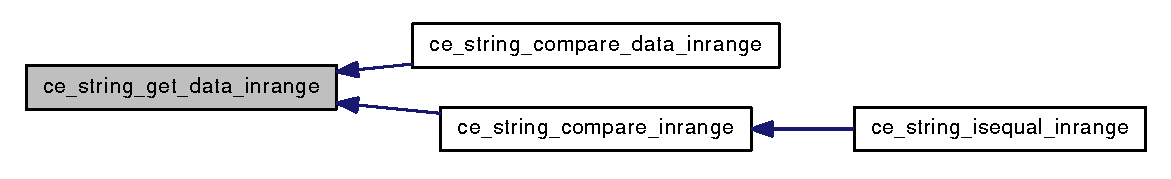
\includegraphics[width=291pt]{cestring_8h_af96303ecd1967b0cc3840ec9f996711e_icgraph}
\end{center}
\end{figure}
\hypertarget{cestring_8h_a91df9c19bf65e917a496a7820d2a3d24}{
\index{cestring.h@{cestring.h}!ce\_\-string\_\-get\_\-length@{ce\_\-string\_\-get\_\-length}}
\index{ce\_\-string\_\-get\_\-length@{ce\_\-string\_\-get\_\-length}!cestring.h@{cestring.h}}
\subsubsection[{ce\_\-string\_\-get\_\-length}]{\setlength{\rightskip}{0pt plus 5cm}{\bf CeInt} ce\_\-string\_\-get\_\-length (CeString $\ast$ {\em self})\hspace{0.3cm}{\ttfamily  \mbox{[}inline\mbox{]}}}}
\label{cestring_8h_a91df9c19bf65e917a496a7820d2a3d24}


Get the length of CeString Object. 
\begin{DoxyParams}{Parameters}
\item[{\em self}]The CeString Object\end{DoxyParams}
\begin{DoxyReturn}{Returns}
The length of CeString Object 
\end{DoxyReturn}


Definition at line 223 of file cestring.c.


\begin{DoxyCode}
224 {
225         return (self->len);
226 }
\end{DoxyCode}
\hypertarget{cestring_8h_ad0580dc439304986492a56145998af96}{
\index{cestring.h@{cestring.h}!ce\_\-string\_\-get\_\-length\_\-inrange@{ce\_\-string\_\-get\_\-length\_\-inrange}}
\index{ce\_\-string\_\-get\_\-length\_\-inrange@{ce\_\-string\_\-get\_\-length\_\-inrange}!cestring.h@{cestring.h}}
\subsubsection[{ce\_\-string\_\-get\_\-length\_\-inrange}]{\setlength{\rightskip}{0pt plus 5cm}{\bf CeInt} ce\_\-string\_\-get\_\-length\_\-inrange (CeString $\ast$ {\em self}, \/  {\bf CeInt} {\em start}, \/  {\bf CeInt} {\em end})}}
\label{cestring_8h_ad0580dc439304986492a56145998af96}


Get the length of CeString Object in range. 
\begin{DoxyParams}{Parameters}
\item[{\em self    The}]CeString Object \item[{\em start}]The first char is 1, the second is 2, blah blah blah. \item[{\em end}]The last char is -\/1 or the length of String Object\end{DoxyParams}
\begin{DoxyReturn}{Returns}
The length of CeString Object in range 
\end{DoxyReturn}


Definition at line 237 of file cestring.c.

References CE\_\-RANGE\_\-INITIAL.


\begin{DoxyCode}
238 {
239         CE_RANGE_INITIAL(start, end, self->len);
240 
241         return (end - start + 1);
242 }
\end{DoxyCode}
\hypertarget{cestring_8h_a11d51db140870c9a79ea20c3c376ca90}{
\index{cestring.h@{cestring.h}!ce\_\-string\_\-isequal@{ce\_\-string\_\-isequal}}
\index{ce\_\-string\_\-isequal@{ce\_\-string\_\-isequal}!cestring.h@{cestring.h}}
\subsubsection[{ce\_\-string\_\-isequal}]{\setlength{\rightskip}{0pt plus 5cm}{\bf CeBool} ce\_\-string\_\-isequal (CeString $\ast$ {\em selfA}, \/  CeString $\ast$ {\em selfB})\hspace{0.3cm}{\ttfamily  \mbox{[}inline\mbox{]}}}}
\label{cestring_8h_a11d51db140870c9a79ea20c3c376ca90}


Test if two CeString Object is equal or not. 
\begin{DoxyParams}{Parameters}
\item[{\em selfA}]A CeString Object \item[{\em selfB}]A CeString Object\end{DoxyParams}
\begin{DoxyReturn}{Returns}
if equal : CE\_\-TRUE else : CE\_\-FALSE 
\end{DoxyReturn}


Definition at line 446 of file cestring.c.

References CE\_\-FALSE, ce\_\-string\_\-compare(), and CE\_\-TRUE.


\begin{DoxyCode}
447 {
448         int resault = ce_string_compare(selfA, selfB);
449 
450         if ( !resault ) {
451                 return CE_TRUE;
452         }
453         else {
454                 return CE_FALSE;
455         }
456 }
\end{DoxyCode}


Here is the call graph for this function:\nopagebreak
\begin{figure}[H]
\begin{center}
\leavevmode
\includegraphics[width=144pt]{cestring_8h_a11d51db140870c9a79ea20c3c376ca90_cgraph}
\end{center}
\end{figure}
\hypertarget{cestring_8h_a36b8df69f79f82c51daa26c5ede8714d}{
\index{cestring.h@{cestring.h}!ce\_\-string\_\-isequal\_\-inrange@{ce\_\-string\_\-isequal\_\-inrange}}
\index{ce\_\-string\_\-isequal\_\-inrange@{ce\_\-string\_\-isequal\_\-inrange}!cestring.h@{cestring.h}}
\subsubsection[{ce\_\-string\_\-isequal\_\-inrange}]{\setlength{\rightskip}{0pt plus 5cm}{\bf CeBool} ce\_\-string\_\-isequal\_\-inrange (CeString $\ast$ {\em selfA}, \/  CeString $\ast$ {\em selfB}, \/  {\bf CeInt} {\em start}, \/  {\bf CeInt} {\em end})\hspace{0.3cm}{\ttfamily  \mbox{[}inline\mbox{]}}}}
\label{cestring_8h_a36b8df69f79f82c51daa26c5ede8714d}


Test if two CeString Object is equal or not in range. 
\begin{DoxyParams}{Parameters}
\item[{\em selfA}]A CeString Object \item[{\em selfB}]A CeString Object \item[{\em start}]The first char is 1, the second is 2, blah blah blah. \item[{\em end}]The last char is -\/1 or the length of String Object\end{DoxyParams}
\begin{DoxyReturn}{Returns}
if equal : CE\_\-TRUE else : CE\_\-FALSE 
\end{DoxyReturn}


Definition at line 470 of file cestring.c.

References CE\_\-FALSE, ce\_\-string\_\-compare\_\-inrange(), and CE\_\-TRUE.


\begin{DoxyCode}
471 {
472         int resault = ce_string_compare_inrange(selfA, selfB, start, end);
473 
474         if ( !resault ) {
475                 return CE_TRUE;
476         }
477         else {
478                 return CE_FALSE;
479         }
480 }
\end{DoxyCode}


Here is the call graph for this function:\nopagebreak
\begin{figure}[H]
\begin{center}
\leavevmode
\includegraphics[width=278pt]{cestring_8h_a36b8df69f79f82c51daa26c5ede8714d_cgraph}
\end{center}
\end{figure}
\hypertarget{cestring_8h_a4bb703271a09a5e293dc117d88a70859}{
\index{cestring.h@{cestring.h}!ce\_\-string\_\-new@{ce\_\-string\_\-new}}
\index{ce\_\-string\_\-new@{ce\_\-string\_\-new}!cestring.h@{cestring.h}}
\subsubsection[{ce\_\-string\_\-new}]{\setlength{\rightskip}{0pt plus 5cm}CeString$\ast$ ce\_\-string\_\-new (void)}}
\label{cestring_8h_a4bb703271a09a5e293dc117d88a70859}


Initial the CeString Object without setting any data. \begin{DoxyReturn}{Returns}
The CeString Object 
\end{DoxyReturn}


Definition at line 54 of file cestring.c.

References CE\_\-STRING\_\-INITIAL.

Referenced by ce\_\-string\_\-new\_\-with\_\-data(), and ce\_\-string\_\-new\_\-with\_\-data\_\-inrange().


\begin{DoxyCode}
55 {
56         CeString *self  = (CeString *) malloc( sizeof(CeString) );
57 
58         if(!selfp) {
59                 selfp  = (CeStringP *) malloc( sizeof(CeStringP) );        
60         }
61 
62         CE_STRING_INITIAL();
63 
64         selfp->data = NULL;
65         selfp->len = 0;
66 
67         return self;
68 }
\end{DoxyCode}


Here is the caller graph for this function:\nopagebreak
\begin{figure}[H]
\begin{center}
\leavevmode
\includegraphics[width=276pt]{cestring_8h_a4bb703271a09a5e293dc117d88a70859_icgraph}
\end{center}
\end{figure}
\hypertarget{cestring_8h_a7704777af405d550d10f1ddd13a525a3}{
\index{cestring.h@{cestring.h}!ce\_\-string\_\-new\_\-with\_\-data@{ce\_\-string\_\-new\_\-with\_\-data}}
\index{ce\_\-string\_\-new\_\-with\_\-data@{ce\_\-string\_\-new\_\-with\_\-data}!cestring.h@{cestring.h}}
\subsubsection[{ce\_\-string\_\-new\_\-with\_\-data}]{\setlength{\rightskip}{0pt plus 5cm}CeString$\ast$ ce\_\-string\_\-new\_\-with\_\-data (const {\bf CeUChar} $\ast$ {\em data})}}
\label{cestring_8h_a7704777af405d550d10f1ddd13a525a3}


Initial the CeString Object and set the data and length. 
\begin{DoxyParams}{Parameters}
\item[{\em data}]A String Object\end{DoxyParams}
\begin{DoxyReturn}{Returns}
The CeString Object 
\end{DoxyReturn}


Definition at line 77 of file cestring.c.

References ce\_\-string\_\-new(), and ce\_\-string\_\-set\_\-data().


\begin{DoxyCode}
78 {
79         CeString *self  = ce_string_new();
80 
81         return ce_string_set_data(self, data);
82 }
\end{DoxyCode}


Here is the call graph for this function:\nopagebreak
\begin{figure}[H]
\begin{center}
\leavevmode
\includegraphics[width=254pt]{cestring_8h_a7704777af405d550d10f1ddd13a525a3_cgraph}
\end{center}
\end{figure}
\hypertarget{cestring_8h_a6e5ca12697c2131bbaa66bbc7bfd7ae5}{
\index{cestring.h@{cestring.h}!ce\_\-string\_\-new\_\-with\_\-data\_\-inrange@{ce\_\-string\_\-new\_\-with\_\-data\_\-inrange}}
\index{ce\_\-string\_\-new\_\-with\_\-data\_\-inrange@{ce\_\-string\_\-new\_\-with\_\-data\_\-inrange}!cestring.h@{cestring.h}}
\subsubsection[{ce\_\-string\_\-new\_\-with\_\-data\_\-inrange}]{\setlength{\rightskip}{0pt plus 5cm}CeString$\ast$ ce\_\-string\_\-new\_\-with\_\-data\_\-inrange (const {\bf CeUChar} $\ast$ {\em data}, \/  {\bf CeInt} {\em start}, \/  {\bf CeInt} {\em end})}}
\label{cestring_8h_a6e5ca12697c2131bbaa66bbc7bfd7ae5}


Initial the CeString Object and set the data in range. 
\begin{DoxyParams}{Parameters}
\item[{\em data}]A String Object \item[{\em start}]The first char is 1, the second is 2, blah blah blah. \item[{\em end}]The last char is -\/1 or the length of String Object.\end{DoxyParams}
\begin{DoxyReturn}{Returns}
The CeString Object 
\end{DoxyReturn}


Definition at line 93 of file cestring.c.

References ce\_\-string\_\-new(), and ce\_\-string\_\-set\_\-data\_\-inrange().

Referenced by ce\_\-string\_\-compare\_\-data\_\-inrange().


\begin{DoxyCode}
94 {
95         CeString *self  = ce_string_new();
96 
97         return ce_string_set_data_inrange(self, data, start, end);
98 }
\end{DoxyCode}


Here is the call graph for this function:\nopagebreak
\begin{figure}[H]
\begin{center}
\leavevmode
\includegraphics[width=202pt]{cestring_8h_a6e5ca12697c2131bbaa66bbc7bfd7ae5_cgraph}
\end{center}
\end{figure}


Here is the caller graph for this function:\nopagebreak
\begin{figure}[H]
\begin{center}
\leavevmode
\includegraphics[width=216pt]{cestring_8h_a6e5ca12697c2131bbaa66bbc7bfd7ae5_icgraph}
\end{center}
\end{figure}
\hypertarget{cestring_8h_a9b450df76273fa5d392a56801554bac4}{
\index{cestring.h@{cestring.h}!ce\_\-string\_\-reverse@{ce\_\-string\_\-reverse}}
\index{ce\_\-string\_\-reverse@{ce\_\-string\_\-reverse}!cestring.h@{cestring.h}}
\subsubsection[{ce\_\-string\_\-reverse}]{\setlength{\rightskip}{0pt plus 5cm}CeString$\ast$ ce\_\-string\_\-reverse (CeString $\ast$ {\em self})\hspace{0.3cm}{\ttfamily  \mbox{[}inline\mbox{]}}}}
\label{cestring_8h_a9b450df76273fa5d392a56801554bac4}


Reverse the data in CeString Object. 
\begin{DoxyParams}{Parameters}
\item[{\em self}]The CeString Object\end{DoxyParams}
\begin{DoxyReturn}{Returns}
The CeString Object 
\end{DoxyReturn}


Definition at line 252 of file cestring.c.

References ce\_\-string\_\-reverse\_\-inrange().


\begin{DoxyCode}
253 {
254         return ce_string_reverse_inrange(self, 1, -1);
255 }
\end{DoxyCode}


Here is the call graph for this function:\nopagebreak
\begin{figure}[H]
\begin{center}
\leavevmode
\includegraphics[width=162pt]{cestring_8h_a9b450df76273fa5d392a56801554bac4_cgraph}
\end{center}
\end{figure}
\hypertarget{cestring_8h_a4fdcc021dd2f1f49e4caf71374a42ef0}{
\index{cestring.h@{cestring.h}!ce\_\-string\_\-reverse\_\-inrange@{ce\_\-string\_\-reverse\_\-inrange}}
\index{ce\_\-string\_\-reverse\_\-inrange@{ce\_\-string\_\-reverse\_\-inrange}!cestring.h@{cestring.h}}
\subsubsection[{ce\_\-string\_\-reverse\_\-inrange}]{\setlength{\rightskip}{0pt plus 5cm}CeString$\ast$ ce\_\-string\_\-reverse\_\-inrange (CeString $\ast$ {\em self}, \/  {\bf CeInt} {\em start}, \/  {\bf CeInt} {\em end})}}
\label{cestring_8h_a4fdcc021dd2f1f49e4caf71374a42ef0}


Reverse the data in CeString Object in range. 
\begin{DoxyParams}{Parameters}
\item[{\em self}]The CeString Object \item[{\em start}]The first char is 1, the second is 2, blah blah blah. \item[{\em end}]The last char is -\/1 or the length of String Object\end{DoxyParams}
\begin{DoxyReturn}{Returns}
The CeString Object 
\end{DoxyReturn}


Definition at line 266 of file cestring.c.

References CE\_\-RANGE\_\-INITIAL, and CE\_\-STRING\_\-INITIAL.

Referenced by ce\_\-string\_\-reverse().


\begin{DoxyCode}
267 {
268         CE_STRING_INITIAL();
269 
270         if ( 1 == selfp->len) {
271                 return self;
272         }
273 
274         CE_RANGE_INITIAL(start, end, self->len);
275 
276         CeInt i = 0;
277         CeInt tmp_len = (end - start) / 2;
278         CeUChar tmp_data;
279 
280         for(; i <= tmp_len; i++) {
281                 tmp_data = selfp->data[i + start];
282                 selfp->data[i + start] = selfp->data[end - i];
283                 selfp->data[end - i] = tmp_data;
284         }
285 
286         return self;
287 }
\end{DoxyCode}


Here is the caller graph for this function:\nopagebreak
\begin{figure}[H]
\begin{center}
\leavevmode
\includegraphics[width=162pt]{cestring_8h_a4fdcc021dd2f1f49e4caf71374a42ef0_icgraph}
\end{center}
\end{figure}
\hypertarget{cestring_8h_a6247e889bdde85791800b881bab0f7f2}{
\index{cestring.h@{cestring.h}!ce\_\-string\_\-set\_\-data@{ce\_\-string\_\-set\_\-data}}
\index{ce\_\-string\_\-set\_\-data@{ce\_\-string\_\-set\_\-data}!cestring.h@{cestring.h}}
\subsubsection[{ce\_\-string\_\-set\_\-data}]{\setlength{\rightskip}{0pt plus 5cm}CeString$\ast$ ce\_\-string\_\-set\_\-data (CeString $\ast$ {\em self}, \/  const {\bf CeUChar} $\ast$ {\em data})\hspace{0.3cm}{\ttfamily  \mbox{[}inline\mbox{]}}}}
\label{cestring_8h_a6247e889bdde85791800b881bab0f7f2}


Setting the data in CeString Object. 
\begin{DoxyParams}{Parameters}
\item[{\em self}]The CeString Object \item[{\em data}]A string that you want to put in CeString Object\end{DoxyParams}
\begin{DoxyReturn}{Returns}
The CeString Object 
\end{DoxyReturn}


Definition at line 138 of file cestring.c.

References ce\_\-string\_\-set\_\-data\_\-inrange().

Referenced by ce\_\-string\_\-append\_\-data\_\-inrange(), ce\_\-string\_\-concat\_\-data\_\-inrange(), and ce\_\-string\_\-new\_\-with\_\-data().


\begin{DoxyCode}
139 {
140         return ce_string_set_data_inrange(self, data, 1, -1);
141 }
\end{DoxyCode}


Here is the call graph for this function:\nopagebreak
\begin{figure}[H]
\begin{center}
\leavevmode
\includegraphics[width=168pt]{cestring_8h_a6247e889bdde85791800b881bab0f7f2_cgraph}
\end{center}
\end{figure}


Here is the caller graph for this function:\nopagebreak
\begin{figure}[H]
\begin{center}
\leavevmode
\includegraphics[width=268pt]{cestring_8h_a6247e889bdde85791800b881bab0f7f2_icgraph}
\end{center}
\end{figure}
\hypertarget{cestring_8h_a5c2a65b88204cb5b8c59f735cac626f9}{
\index{cestring.h@{cestring.h}!ce\_\-string\_\-set\_\-data\_\-inrange@{ce\_\-string\_\-set\_\-data\_\-inrange}}
\index{ce\_\-string\_\-set\_\-data\_\-inrange@{ce\_\-string\_\-set\_\-data\_\-inrange}!cestring.h@{cestring.h}}
\subsubsection[{ce\_\-string\_\-set\_\-data\_\-inrange}]{\setlength{\rightskip}{0pt plus 5cm}CeString$\ast$ ce\_\-string\_\-set\_\-data\_\-inrange (CeString $\ast$ {\em self}, \/  const {\bf CeUChar} $\ast$ {\em data}, \/  {\bf CeInt} {\em start}, \/  {\bf CeInt} {\em end})}}
\label{cestring_8h_a5c2a65b88204cb5b8c59f735cac626f9}


Setting the data in range in CeString Object. 
\begin{DoxyParams}{Parameters}
\item[{\em self}]The CeString Object \item[{\em data}]A String Object \item[{\em start}]The first char is 1, the second is 2, blah blah blah. \item[{\em end}]The last char is -\/1 or the length of String Object\end{DoxyParams}
\begin{DoxyReturn}{Returns}
The CeString Object 
\end{DoxyReturn}


Definition at line 153 of file cestring.c.

References CE\_\-RANGE\_\-INITIAL, and CE\_\-STRING\_\-INITIAL.

Referenced by ce\_\-string\_\-copy\_\-inrange(), ce\_\-string\_\-new\_\-with\_\-data\_\-inrange(), and ce\_\-string\_\-set\_\-data().


\begin{DoxyCode}
154 {
155         CE_STRING_INITIAL();
156 
157         CeInt length = strlen(data);
158 
159         CE_RANGE_INITIAL(start, end, length);
160 
161         length = end - start + 1;
162         
163         /* Free the CeString Object first */
164         if(0 != selfp->len) {
165                 free(self->data);
166         }
167 
168         selfp->len = length;
169         selfp->data = (CeUChar *) malloc( sizeof(CeUChar) * (length + 1) );
170         
171         /* Now let's copy new string to our CeString */
172         memcpy(selfp->data, data + start, length);
173         selfp->data[length] = '\0';   /* end of line */
174 
175         return self;
176 }
\end{DoxyCode}


Here is the caller graph for this function:\nopagebreak
\begin{figure}[H]
\begin{center}
\leavevmode
\includegraphics[width=397pt]{cestring_8h_a5c2a65b88204cb5b8c59f735cac626f9_icgraph}
\end{center}
\end{figure}
\hypertarget{cestring_8h_a953a69047221ef6d7fdc32f2a8f5bcf3}{
\index{cestring.h@{cestring.h}!ce\_\-string\_\-swap@{ce\_\-string\_\-swap}}
\index{ce\_\-string\_\-swap@{ce\_\-string\_\-swap}!cestring.h@{cestring.h}}
\subsubsection[{ce\_\-string\_\-swap}]{\setlength{\rightskip}{0pt plus 5cm}void ce\_\-string\_\-swap (CeString $\ast$ {\em selfA}, \/  CeString $\ast$ {\em selfB})\hspace{0.3cm}{\ttfamily  \mbox{[}inline\mbox{]}}}}
\label{cestring_8h_a953a69047221ef6d7fdc32f2a8f5bcf3}


Swap two CeString Object. 
\begin{DoxyParams}{Parameters}
\item[{\em selfA}]A CeString Object \item[{\em selfB}]A CeString Object \end{DoxyParams}


Definition at line 521 of file cestring.c.


\begin{DoxyCode}
522 {
523         selfp = (CeStringP *) selfA;
524         selfA = selfB;
525         selfB = (CeString  *) selfp;
526 }
\end{DoxyCode}
\hypertarget{cestring_8h_aee10e1e7cc9de8fd7590eab96c630538}{
\index{cestring.h@{cestring.h}!ce\_\-string\_\-tolower@{ce\_\-string\_\-tolower}}
\index{ce\_\-string\_\-tolower@{ce\_\-string\_\-tolower}!cestring.h@{cestring.h}}
\subsubsection[{ce\_\-string\_\-tolower}]{\setlength{\rightskip}{0pt plus 5cm}CeString$\ast$ ce\_\-string\_\-tolower (CeString $\ast$ {\em self})\hspace{0.3cm}{\ttfamily  \mbox{[}inline\mbox{]}}}}
\label{cestring_8h_aee10e1e7cc9de8fd7590eab96c630538}


Make all the cahracters in CeString object to lowercase. 
\begin{DoxyParams}{Parameters}
\item[{\em self}]The CeString Object\end{DoxyParams}
\begin{DoxyReturn}{Returns}
The CeString Object 
\end{DoxyReturn}


Definition at line 334 of file cestring.c.

References ce\_\-string\_\-tolower\_\-inrange().


\begin{DoxyCode}
335 {
336         return ce_string_tolower_inrange(self, 1, -1);
337 }
\end{DoxyCode}


Here is the call graph for this function:\nopagebreak
\begin{figure}[H]
\begin{center}
\leavevmode
\includegraphics[width=161pt]{cestring_8h_aee10e1e7cc9de8fd7590eab96c630538_cgraph}
\end{center}
\end{figure}
\hypertarget{cestring_8h_ac2652db2d918411eb362eb1998d9b81c}{
\index{cestring.h@{cestring.h}!ce\_\-string\_\-tolower\_\-inrange@{ce\_\-string\_\-tolower\_\-inrange}}
\index{ce\_\-string\_\-tolower\_\-inrange@{ce\_\-string\_\-tolower\_\-inrange}!cestring.h@{cestring.h}}
\subsubsection[{ce\_\-string\_\-tolower\_\-inrange}]{\setlength{\rightskip}{0pt plus 5cm}CeString$\ast$ ce\_\-string\_\-tolower\_\-inrange (CeString $\ast$ {\em self}, \/  {\bf CeInt} {\em start}, \/  {\bf CeInt} {\em end})}}
\label{cestring_8h_ac2652db2d918411eb362eb1998d9b81c}


Make the cahracters in CeString object in range to lowercase. 
\begin{DoxyParams}{Parameters}
\item[{\em self}]The CeString Object \item[{\em start}]The first char is 1, the second is 2, blah blah blah. \item[{\em end}]The last char is -\/1 or the length of String Object\end{DoxyParams}
\begin{DoxyReturn}{Returns}
The CeString Object 
\end{DoxyReturn}


Definition at line 348 of file cestring.c.

References CE\_\-RANGE\_\-INITIAL, and CE\_\-STRING\_\-INITIAL.

Referenced by ce\_\-string\_\-tolower().


\begin{DoxyCode}
349 {
350         CE_STRING_INITIAL();
351 
352         CE_RANGE_INITIAL(start, end, self->len);
353         
354         CeInt i = start;
355 
356         for (; i <= end; i++) {
357                 selfp->data[i] = tolower(selfp->data[i]);
358         }
359 
360         return self;
361 }
\end{DoxyCode}


Here is the caller graph for this function:\nopagebreak
\begin{figure}[H]
\begin{center}
\leavevmode
\includegraphics[width=161pt]{cestring_8h_ac2652db2d918411eb362eb1998d9b81c_icgraph}
\end{center}
\end{figure}
\hypertarget{cestring_8h_ad1a2462f927173410b6ef2cf1bc0a9c8}{
\index{cestring.h@{cestring.h}!ce\_\-string\_\-toupper@{ce\_\-string\_\-toupper}}
\index{ce\_\-string\_\-toupper@{ce\_\-string\_\-toupper}!cestring.h@{cestring.h}}
\subsubsection[{ce\_\-string\_\-toupper}]{\setlength{\rightskip}{0pt plus 5cm}CeString$\ast$ ce\_\-string\_\-toupper (CeString $\ast$ {\em self})\hspace{0.3cm}{\ttfamily  \mbox{[}inline\mbox{]}}}}
\label{cestring_8h_ad1a2462f927173410b6ef2cf1bc0a9c8}


Make all the cahracters in CeString object to uppercase. 
\begin{DoxyParams}{Parameters}
\item[{\em self}]The CeString Object\end{DoxyParams}
\begin{DoxyReturn}{Returns}
The CeString Object 
\end{DoxyReturn}


Definition at line 297 of file cestring.c.

References ce\_\-string\_\-toupper\_\-inrange().


\begin{DoxyCode}
298 {
299         return ce_string_toupper_inrange(self, 1, -1);
300 }
\end{DoxyCode}


Here is the call graph for this function:\nopagebreak
\begin{figure}[H]
\begin{center}
\leavevmode
\includegraphics[width=163pt]{cestring_8h_ad1a2462f927173410b6ef2cf1bc0a9c8_cgraph}
\end{center}
\end{figure}
\hypertarget{cestring_8h_ae75eae2ff0d6ffd505f35c9b073353b4}{
\index{cestring.h@{cestring.h}!ce\_\-string\_\-toupper\_\-inrange@{ce\_\-string\_\-toupper\_\-inrange}}
\index{ce\_\-string\_\-toupper\_\-inrange@{ce\_\-string\_\-toupper\_\-inrange}!cestring.h@{cestring.h}}
\subsubsection[{ce\_\-string\_\-toupper\_\-inrange}]{\setlength{\rightskip}{0pt plus 5cm}CeString$\ast$ ce\_\-string\_\-toupper\_\-inrange (CeString $\ast$ {\em self}, \/  {\bf CeInt} {\em start}, \/  {\bf CeInt} {\em end})}}
\label{cestring_8h_ae75eae2ff0d6ffd505f35c9b073353b4}


Make the cahracters in CeString object in range to uppercase. 
\begin{DoxyParams}{Parameters}
\item[{\em self}]The CeString Object \item[{\em start}]The first char is 1, the second is 2, blah blah blah. \item[{\em end}]The last char is -\/1 or the length of String Object\end{DoxyParams}
\begin{DoxyReturn}{Returns}
The CeString Object 
\end{DoxyReturn}


Definition at line 311 of file cestring.c.

References CE\_\-RANGE\_\-INITIAL, and CE\_\-STRING\_\-INITIAL.

Referenced by ce\_\-string\_\-toupper().


\begin{DoxyCode}
312 {
313         CE_STRING_INITIAL();
314 
315         CE_RANGE_INITIAL(start, end, self->len);
316 
317         CeInt i = start;
318 
319         for (; i <= end; i++) {
320                 selfp->data[i] = toupper(selfp->data[i]);
321         }
322 
323         return self;
324 }
\end{DoxyCode}


Here is the caller graph for this function:\nopagebreak
\begin{figure}[H]
\begin{center}
\leavevmode
\includegraphics[width=163pt]{cestring_8h_ae75eae2ff0d6ffd505f35c9b073353b4_icgraph}
\end{center}
\end{figure}

\hypertarget{ceswap_8c}{
\section{src/ceswap.c File Reference}
\label{ceswap_8c}\index{src/ceswap.c@{src/ceswap.c}}
}
{\ttfamily \#include $<$stdio.h$>$}\par
{\ttfamily \#include \char`\"{}cetypes.h\char`\"{}}\par
{\ttfamily \#include \char`\"{}ceswap.h\char`\"{}}\par
Include dependency graph for ceswap.c:\nopagebreak
\begin{figure}[H]
\begin{center}
\leavevmode
\includegraphics[width=125pt]{ceswap_8c__incl}
\end{center}
\end{figure}
\subsection*{Defines}
\begin{DoxyCompactItemize}
\item 
\#define \hyperlink{ceswap_8c_aa31315169cc31c256b6997949825818e}{CE\_\-SWAP\_\-CORE}~tmp = $\ast$p1; $\ast$p1 = $\ast$p2; $\ast$p2 = tmp
\end{DoxyCompactItemize}
\subsection*{Functions}
\begin{DoxyCompactItemize}
\item 
void \hyperlink{ceswap_8c_a214de63cdec3f218cec2216c7d5161ac}{ce\_\-int\_\-swap} (\hyperlink{cetypes_8h_aced3fca6c74c98a0a7c07757af07abca}{CeInt} $\ast$p1, \hyperlink{cetypes_8h_aced3fca6c74c98a0a7c07757af07abca}{CeInt} $\ast$p2)
\item 
void \hyperlink{ceswap_8c_a3605edd83248b6c3dfc7fb1fe069cd7e}{ce\_\-char\_\-swap} (\hyperlink{cetypes_8h_a8512a2734cab1f8c3592edade4b821b0}{CeChar} $\ast$p1, \hyperlink{cetypes_8h_a8512a2734cab1f8c3592edade4b821b0}{CeChar} $\ast$p2)
\item 
void \hyperlink{ceswap_8c_ab01d652f6cf8002d1f0736f85d884e52}{ce\_\-short\_\-swap} (\hyperlink{cetypes_8h_ae6af6dd3ddf122e15e79db603d81cb16}{CeShort} $\ast$p1, \hyperlink{cetypes_8h_ae6af6dd3ddf122e15e79db603d81cb16}{CeShort} $\ast$p2)
\item 
void \hyperlink{ceswap_8c_ae5fca3375ad51efb7b3f8319b6095b74}{ce\_\-float\_\-swap} (\hyperlink{cetypes_8h_a09f99756f4fd45fba87dda233ffbc311}{CeFloat} $\ast$p1, \hyperlink{cetypes_8h_a09f99756f4fd45fba87dda233ffbc311}{CeFloat} $\ast$p2)
\item 
void \hyperlink{ceswap_8c_af8933749dfd36d98b27756e70ef775d2}{ce\_\-double\_\-swap} (\hyperlink{cetypes_8h_a8f09afda6e020579a7fdefcf032cebf8}{CeDouble} $\ast$p1, \hyperlink{cetypes_8h_a8f09afda6e020579a7fdefcf032cebf8}{CeDouble} $\ast$p2)
\item 
void \hyperlink{ceswap_8c_a01cc20014ca247d2e94009d23ce37a15}{ce\_\-uint\_\-swap} (\hyperlink{cetypes_8h_a27dd20f82b38cab490e94d8fe9924905}{CeUInt} $\ast$p1, \hyperlink{cetypes_8h_a27dd20f82b38cab490e94d8fe9924905}{CeUInt} $\ast$p2)
\item 
void \hyperlink{ceswap_8c_ae7350b79b1e8103161209ce4893180c6}{ce\_\-uchar\_\-swap} (\hyperlink{cetypes_8h_a3a94319866313b53b54825af2ba77e8d}{CeUChar} $\ast$p1, \hyperlink{cetypes_8h_a3a94319866313b53b54825af2ba77e8d}{CeUChar} $\ast$p2)
\item 
void \hyperlink{ceswap_8c_a10a8e51c5b14b80e99423ecc401ee419}{ce\_\-ushort\_\-swap} (\hyperlink{cetypes_8h_a6f3fba70e7c0908171a8ba737c217b76}{CeUShort} $\ast$p1, \hyperlink{cetypes_8h_a6f3fba70e7c0908171a8ba737c217b76}{CeUShort} $\ast$p2)
\end{DoxyCompactItemize}


\subsection{Define Documentation}
\hypertarget{ceswap_8c_aa31315169cc31c256b6997949825818e}{
\index{ceswap.c@{ceswap.c}!CE\_\-SWAP\_\-CORE@{CE\_\-SWAP\_\-CORE}}
\index{CE\_\-SWAP\_\-CORE@{CE\_\-SWAP\_\-CORE}!ceswap.c@{ceswap.c}}
\subsubsection[{CE\_\-SWAP\_\-CORE}]{\setlength{\rightskip}{0pt plus 5cm}\#define CE\_\-SWAP\_\-CORE~tmp = $\ast$p1; $\ast$p1 = $\ast$p2; $\ast$p2 = tmp}}
\label{ceswap_8c_aa31315169cc31c256b6997949825818e}


Definition at line 29 of file ceswap.c.

Referenced by ce\_\-char\_\-swap(), ce\_\-double\_\-swap(), ce\_\-float\_\-swap(), ce\_\-int\_\-swap(), ce\_\-short\_\-swap(), ce\_\-uchar\_\-swap(), ce\_\-uint\_\-swap(), and ce\_\-ushort\_\-swap().

\subsection{Function Documentation}
\hypertarget{ceswap_8c_a3605edd83248b6c3dfc7fb1fe069cd7e}{
\index{ceswap.c@{ceswap.c}!ce\_\-char\_\-swap@{ce\_\-char\_\-swap}}
\index{ce\_\-char\_\-swap@{ce\_\-char\_\-swap}!ceswap.c@{ceswap.c}}
\subsubsection[{ce\_\-char\_\-swap}]{\setlength{\rightskip}{0pt plus 5cm}void ce\_\-char\_\-swap ({\bf CeChar} $\ast$ {\em p1}, \/  {\bf CeChar} $\ast$ {\em p2})\hspace{0.3cm}{\ttfamily  \mbox{[}inline\mbox{]}}}}
\label{ceswap_8c_a3605edd83248b6c3dfc7fb1fe069cd7e}


Definition at line 38 of file ceswap.c.

References CE\_\-SWAP\_\-CORE.


\begin{DoxyCode}
39 {
40         CeChar CE_SWAP_CORE;
41 }
\end{DoxyCode}
\hypertarget{ceswap_8c_af8933749dfd36d98b27756e70ef775d2}{
\index{ceswap.c@{ceswap.c}!ce\_\-double\_\-swap@{ce\_\-double\_\-swap}}
\index{ce\_\-double\_\-swap@{ce\_\-double\_\-swap}!ceswap.c@{ceswap.c}}
\subsubsection[{ce\_\-double\_\-swap}]{\setlength{\rightskip}{0pt plus 5cm}void ce\_\-double\_\-swap ({\bf CeDouble} $\ast$ {\em p1}, \/  {\bf CeDouble} $\ast$ {\em p2})\hspace{0.3cm}{\ttfamily  \mbox{[}inline\mbox{]}}}}
\label{ceswap_8c_af8933749dfd36d98b27756e70ef775d2}


Definition at line 56 of file ceswap.c.

References CE\_\-SWAP\_\-CORE.


\begin{DoxyCode}
57 {
58         CeDouble CE_SWAP_CORE;
59 }
\end{DoxyCode}
\hypertarget{ceswap_8c_ae5fca3375ad51efb7b3f8319b6095b74}{
\index{ceswap.c@{ceswap.c}!ce\_\-float\_\-swap@{ce\_\-float\_\-swap}}
\index{ce\_\-float\_\-swap@{ce\_\-float\_\-swap}!ceswap.c@{ceswap.c}}
\subsubsection[{ce\_\-float\_\-swap}]{\setlength{\rightskip}{0pt plus 5cm}void ce\_\-float\_\-swap ({\bf CeFloat} $\ast$ {\em p1}, \/  {\bf CeFloat} $\ast$ {\em p2})\hspace{0.3cm}{\ttfamily  \mbox{[}inline\mbox{]}}}}
\label{ceswap_8c_ae5fca3375ad51efb7b3f8319b6095b74}


Definition at line 50 of file ceswap.c.

References CE\_\-SWAP\_\-CORE.


\begin{DoxyCode}
51 {
52         CeFloat CE_SWAP_CORE;
53 }
\end{DoxyCode}
\hypertarget{ceswap_8c_a214de63cdec3f218cec2216c7d5161ac}{
\index{ceswap.c@{ceswap.c}!ce\_\-int\_\-swap@{ce\_\-int\_\-swap}}
\index{ce\_\-int\_\-swap@{ce\_\-int\_\-swap}!ceswap.c@{ceswap.c}}
\subsubsection[{ce\_\-int\_\-swap}]{\setlength{\rightskip}{0pt plus 5cm}void ce\_\-int\_\-swap ({\bf CeInt} $\ast$ {\em p1}, \/  {\bf CeInt} $\ast$ {\em p2})\hspace{0.3cm}{\ttfamily  \mbox{[}inline\mbox{]}}}}
\label{ceswap_8c_a214de63cdec3f218cec2216c7d5161ac}


Definition at line 32 of file ceswap.c.

References CE\_\-SWAP\_\-CORE.


\begin{DoxyCode}
33 {
34         CeInt CE_SWAP_CORE;
35 }
\end{DoxyCode}
\hypertarget{ceswap_8c_ab01d652f6cf8002d1f0736f85d884e52}{
\index{ceswap.c@{ceswap.c}!ce\_\-short\_\-swap@{ce\_\-short\_\-swap}}
\index{ce\_\-short\_\-swap@{ce\_\-short\_\-swap}!ceswap.c@{ceswap.c}}
\subsubsection[{ce\_\-short\_\-swap}]{\setlength{\rightskip}{0pt plus 5cm}void ce\_\-short\_\-swap ({\bf CeShort} $\ast$ {\em p1}, \/  {\bf CeShort} $\ast$ {\em p2})\hspace{0.3cm}{\ttfamily  \mbox{[}inline\mbox{]}}}}
\label{ceswap_8c_ab01d652f6cf8002d1f0736f85d884e52}


Definition at line 44 of file ceswap.c.

References CE\_\-SWAP\_\-CORE.


\begin{DoxyCode}
45 {
46         CeShort CE_SWAP_CORE;
47 }
\end{DoxyCode}
\hypertarget{ceswap_8c_ae7350b79b1e8103161209ce4893180c6}{
\index{ceswap.c@{ceswap.c}!ce\_\-uchar\_\-swap@{ce\_\-uchar\_\-swap}}
\index{ce\_\-uchar\_\-swap@{ce\_\-uchar\_\-swap}!ceswap.c@{ceswap.c}}
\subsubsection[{ce\_\-uchar\_\-swap}]{\setlength{\rightskip}{0pt plus 5cm}void ce\_\-uchar\_\-swap ({\bf CeUChar} $\ast$ {\em p1}, \/  {\bf CeUChar} $\ast$ {\em p2})\hspace{0.3cm}{\ttfamily  \mbox{[}inline\mbox{]}}}}
\label{ceswap_8c_ae7350b79b1e8103161209ce4893180c6}


Definition at line 69 of file ceswap.c.

References CE\_\-SWAP\_\-CORE.


\begin{DoxyCode}
70 {
71         CeUChar CE_SWAP_CORE;
72 }
\end{DoxyCode}
\hypertarget{ceswap_8c_a01cc20014ca247d2e94009d23ce37a15}{
\index{ceswap.c@{ceswap.c}!ce\_\-uint\_\-swap@{ce\_\-uint\_\-swap}}
\index{ce\_\-uint\_\-swap@{ce\_\-uint\_\-swap}!ceswap.c@{ceswap.c}}
\subsubsection[{ce\_\-uint\_\-swap}]{\setlength{\rightskip}{0pt plus 5cm}void ce\_\-uint\_\-swap ({\bf CeUInt} $\ast$ {\em p1}, \/  {\bf CeUInt} $\ast$ {\em p2})\hspace{0.3cm}{\ttfamily  \mbox{[}inline\mbox{]}}}}
\label{ceswap_8c_a01cc20014ca247d2e94009d23ce37a15}


Definition at line 63 of file ceswap.c.

References CE\_\-SWAP\_\-CORE.


\begin{DoxyCode}
64 {
65         CeUInt CE_SWAP_CORE;
66 }
\end{DoxyCode}
\hypertarget{ceswap_8c_a10a8e51c5b14b80e99423ecc401ee419}{
\index{ceswap.c@{ceswap.c}!ce\_\-ushort\_\-swap@{ce\_\-ushort\_\-swap}}
\index{ce\_\-ushort\_\-swap@{ce\_\-ushort\_\-swap}!ceswap.c@{ceswap.c}}
\subsubsection[{ce\_\-ushort\_\-swap}]{\setlength{\rightskip}{0pt plus 5cm}void ce\_\-ushort\_\-swap ({\bf CeUShort} $\ast$ {\em p1}, \/  {\bf CeUShort} $\ast$ {\em p2})\hspace{0.3cm}{\ttfamily  \mbox{[}inline\mbox{]}}}}
\label{ceswap_8c_a10a8e51c5b14b80e99423ecc401ee419}


Definition at line 75 of file ceswap.c.

References CE\_\-SWAP\_\-CORE.


\begin{DoxyCode}
76 {
77         CeUShort CE_SWAP_CORE;
78 }
\end{DoxyCode}

\include{ceswap_8h}
\hypertarget{cetypes_8h}{
\section{src/cetypes.h File Reference}
\label{cetypes_8h}\index{src/cetypes.h@{src/cetypes.h}}
}
This graph shows which files directly or indirectly include this file:\nopagebreak
\begin{figure}[H]
\begin{center}
\leavevmode
\includegraphics[width=109pt]{cetypes_8h__dep__incl}
\end{center}
\end{figure}
\subsection*{Typedefs}
\begin{DoxyCompactItemize}
\item 
typedef int \hyperlink{cetypes_8h_aced3fca6c74c98a0a7c07757af07abca}{CeInt}
\item 
typedef char \hyperlink{cetypes_8h_a8512a2734cab1f8c3592edade4b821b0}{CeChar}
\item 
typedef short \hyperlink{cetypes_8h_a754a1ea7b6bec3cd8d26c3a9794228dc}{CeBool}
\item 
typedef long \hyperlink{cetypes_8h_a5e9425b44e528e8f4e76c1a1d3f220ec}{CeLong}
\item 
typedef short \hyperlink{cetypes_8h_ae6af6dd3ddf122e15e79db603d81cb16}{CeShort}
\item 
typedef unsigned int \hyperlink{cetypes_8h_a27dd20f82b38cab490e94d8fe9924905}{CeUInt}
\item 
typedef unsigned char \hyperlink{cetypes_8h_a3a94319866313b53b54825af2ba77e8d}{CeUChar}
\item 
typedef unsigned long \hyperlink{cetypes_8h_ab818eea25359e419343a4735ad8ba012}{CeULong}
\item 
typedef unsigned short \hyperlink{cetypes_8h_a6f3fba70e7c0908171a8ba737c217b76}{CeUShort}
\item 
typedef float \hyperlink{cetypes_8h_a09f99756f4fd45fba87dda233ffbc311}{CeFloat}
\item 
typedef double \hyperlink{cetypes_8h_a8f09afda6e020579a7fdefcf032cebf8}{CeDouble}
\item 
typedef void $\ast$ \hyperlink{cetypes_8h_a2b9f6f950a83a5a9f2efd68b8b6da296}{CePointer}
\end{DoxyCompactItemize}


\subsection{Typedef Documentation}
\hypertarget{cetypes_8h_a754a1ea7b6bec3cd8d26c3a9794228dc}{
\index{cetypes.h@{cetypes.h}!CeBool@{CeBool}}
\index{CeBool@{CeBool}!cetypes.h@{cetypes.h}}
\subsubsection[{CeBool}]{\setlength{\rightskip}{0pt plus 5cm}typedef short {\bf CeBool}}}
\label{cetypes_8h_a754a1ea7b6bec3cd8d26c3a9794228dc}


Definition at line 34 of file cetypes.h.\hypertarget{cetypes_8h_a8512a2734cab1f8c3592edade4b821b0}{
\index{cetypes.h@{cetypes.h}!CeChar@{CeChar}}
\index{CeChar@{CeChar}!cetypes.h@{cetypes.h}}
\subsubsection[{CeChar}]{\setlength{\rightskip}{0pt plus 5cm}typedef char {\bf CeChar}}}
\label{cetypes_8h_a8512a2734cab1f8c3592edade4b821b0}


Definition at line 33 of file cetypes.h.\hypertarget{cetypes_8h_a8f09afda6e020579a7fdefcf032cebf8}{
\index{cetypes.h@{cetypes.h}!CeDouble@{CeDouble}}
\index{CeDouble@{CeDouble}!cetypes.h@{cetypes.h}}
\subsubsection[{CeDouble}]{\setlength{\rightskip}{0pt plus 5cm}typedef double {\bf CeDouble}}}
\label{cetypes_8h_a8f09afda6e020579a7fdefcf032cebf8}


Definition at line 44 of file cetypes.h.\hypertarget{cetypes_8h_a09f99756f4fd45fba87dda233ffbc311}{
\index{cetypes.h@{cetypes.h}!CeFloat@{CeFloat}}
\index{CeFloat@{CeFloat}!cetypes.h@{cetypes.h}}
\subsubsection[{CeFloat}]{\setlength{\rightskip}{0pt plus 5cm}typedef float {\bf CeFloat}}}
\label{cetypes_8h_a09f99756f4fd45fba87dda233ffbc311}


Definition at line 43 of file cetypes.h.\hypertarget{cetypes_8h_aced3fca6c74c98a0a7c07757af07abca}{
\index{cetypes.h@{cetypes.h}!CeInt@{CeInt}}
\index{CeInt@{CeInt}!cetypes.h@{cetypes.h}}
\subsubsection[{CeInt}]{\setlength{\rightskip}{0pt plus 5cm}typedef int {\bf CeInt}}}
\label{cetypes_8h_aced3fca6c74c98a0a7c07757af07abca}


Definition at line 32 of file cetypes.h.\hypertarget{cetypes_8h_a5e9425b44e528e8f4e76c1a1d3f220ec}{
\index{cetypes.h@{cetypes.h}!CeLong@{CeLong}}
\index{CeLong@{CeLong}!cetypes.h@{cetypes.h}}
\subsubsection[{CeLong}]{\setlength{\rightskip}{0pt plus 5cm}typedef long {\bf CeLong}}}
\label{cetypes_8h_a5e9425b44e528e8f4e76c1a1d3f220ec}


Definition at line 35 of file cetypes.h.\hypertarget{cetypes_8h_a2b9f6f950a83a5a9f2efd68b8b6da296}{
\index{cetypes.h@{cetypes.h}!CePointer@{CePointer}}
\index{CePointer@{CePointer}!cetypes.h@{cetypes.h}}
\subsubsection[{CePointer}]{\setlength{\rightskip}{0pt plus 5cm}typedef void$\ast$ {\bf CePointer}}}
\label{cetypes_8h_a2b9f6f950a83a5a9f2efd68b8b6da296}


Definition at line 46 of file cetypes.h.\hypertarget{cetypes_8h_ae6af6dd3ddf122e15e79db603d81cb16}{
\index{cetypes.h@{cetypes.h}!CeShort@{CeShort}}
\index{CeShort@{CeShort}!cetypes.h@{cetypes.h}}
\subsubsection[{CeShort}]{\setlength{\rightskip}{0pt plus 5cm}typedef short {\bf CeShort}}}
\label{cetypes_8h_ae6af6dd3ddf122e15e79db603d81cb16}


Definition at line 36 of file cetypes.h.\hypertarget{cetypes_8h_a3a94319866313b53b54825af2ba77e8d}{
\index{cetypes.h@{cetypes.h}!CeUChar@{CeUChar}}
\index{CeUChar@{CeUChar}!cetypes.h@{cetypes.h}}
\subsubsection[{CeUChar}]{\setlength{\rightskip}{0pt plus 5cm}typedef unsigned char {\bf CeUChar}}}
\label{cetypes_8h_a3a94319866313b53b54825af2ba77e8d}


Definition at line 39 of file cetypes.h.\hypertarget{cetypes_8h_a27dd20f82b38cab490e94d8fe9924905}{
\index{cetypes.h@{cetypes.h}!CeUInt@{CeUInt}}
\index{CeUInt@{CeUInt}!cetypes.h@{cetypes.h}}
\subsubsection[{CeUInt}]{\setlength{\rightskip}{0pt plus 5cm}typedef unsigned int {\bf CeUInt}}}
\label{cetypes_8h_a27dd20f82b38cab490e94d8fe9924905}


Definition at line 38 of file cetypes.h.\hypertarget{cetypes_8h_ab818eea25359e419343a4735ad8ba012}{
\index{cetypes.h@{cetypes.h}!CeULong@{CeULong}}
\index{CeULong@{CeULong}!cetypes.h@{cetypes.h}}
\subsubsection[{CeULong}]{\setlength{\rightskip}{0pt plus 5cm}typedef unsigned long {\bf CeULong}}}
\label{cetypes_8h_ab818eea25359e419343a4735ad8ba012}


Definition at line 40 of file cetypes.h.\hypertarget{cetypes_8h_a6f3fba70e7c0908171a8ba737c217b76}{
\index{cetypes.h@{cetypes.h}!CeUShort@{CeUShort}}
\index{CeUShort@{CeUShort}!cetypes.h@{cetypes.h}}
\subsubsection[{CeUShort}]{\setlength{\rightskip}{0pt plus 5cm}typedef unsigned short {\bf CeUShort}}}
\label{cetypes_8h_a6f3fba70e7c0908171a8ba737c217b76}


Definition at line 41 of file cetypes.h.
\printindex
\end{document}
